\documentclass[iop,apj]{emulateapj}
\usepackage{amsmath,amssymb,amstext}
\usepackage[breaklinks,colorlinks,citecolor=blue,linkcolor=magenta]{hyperref}
\renewcommand*{\sectionautorefname}{Section}
\usepackage[all]{hypcap} %Links go to figures; breaks on deluxetables (use \capstartfalse \capstarttrue to fix it)
\usepackage[]{algorithm2e}
\usepackage{subfigure}
\usepackage{enumerate}
\usepackage{float}
\usepackage{graphicx}
\usepackage[ampersand]{easylist}
\usepackage{verbatim}
\usepackage{trimclip}

\begin{document}

\title{[Automatic Identification of Spectral Lines through Spectrum Reconstruction]}
\author{Andr\'es Riveros	$^1$}
\author{Karim Pichara		$^{1,5, 2}$}
\author{Pavlos Protopapas	$^2$}
\author{Diego Mardones		$^3$}
\author{Mauricio Araya		$^4$}
\affil{$^1$ Computer Science Department, Pontif\'icia Universidad Cat\'olica de Chile, Santiago, Chile}
\affil{$^2$ Institute for Applied Computational Science, Harvard University, Cambridge, MA, USA}
\affil{$^3$ Astronomy Department, Universidad de Chile, Santiago, Chile}
\affil{$^4$ Computer Science Department, Universidad T\'ecnica Federico Santa Mar\'ia, Valpara\'iso, Chile}
\affil{\altaffilmark{5}Millennium Institute of Astrophysics, Chile}

\begin{abstract}

\begin{comment}
    - Massive Amount of Data
    - Astronomers overloaded
    - What is spectroscopy
    - Need to automatize process
    - Step by step task of astronomer
    - Focus of this work
    - Automatic Proposed Algorithm
    - Detailing Algorithm Operation
    - Reached Results
    - Strengths and limitations
    - Conclusions
\end{comment}


Astronomy is facing new challenges on how to analyze big data and therefore, how to search or predict events/patterns of interest.
New observations in previously unexplored wavelength regions will be available from instruments such as the Atacama Large Millimeter Array (ALMA).
Given this growing amount of high spectral resolution data, any non-automatic analysis would be an effort beyond human's capacity.
Currently, classifying emission lines means to decide if a particular emission line belongs to a specific isotope. 
This classification is mainly done by comparing them with known isotopes emission lines.
An automatic line-classification algorithm would dramatically reduce human efforts to analyze spectral data, allowing astronomers to focus their efforts in deeper analysis.

In this work, we propose an algorithm that uses a sparse model to represent the spectra and automatically classify emission lines.
We use spectral line databases to determine a set of basis vectors that represent the presence of theoretical emission lines.
Then, to classify lines in a given spectrum, the difference between the spectrum and a linear combination of the determined basis vectors is minimized.

The model's output correspond to a probability vector representing the distribution of the prediction over a set of possible isotopes. 
We test our algorithm with experimental data from Splatalogue and simulated data from the ASYDO project.
The results of the analysis show that the algorithm is able to identify emission lines with an accuracy of 90\% when no blending nor hyperfine cases are present.
As wavelength separation decreases (equal or less than $1$ MHz), accuracy goes down to 82\%.

The source code of the algorithm, synthetic data cubes used and list of suggested identifications are publicly available \footnote{https://github.com/ChileanVirtualObservatory/DISPLAY}.

\end{abstract}

\keywords{
    spectral lines: emission lines;
    technique: spectroscopy;
    method: data analysis
    }

\maketitle

\section{Introduction} \label{sec:intro}

% (1 Page)
% Present Tense

\begin{comment}
    - Massive Amount of Data
    - Astronomers overloaded
    - Step by step task of astronomer
    - Need to automatize process
    - Focus of solution
    - Final objective of solution
    - Automatic Proposed Algorithm
    - Algorithm Operation Detail
    - Strengths and limitations
    - Conclusions
    - List of Content
\end{comment}

Modern astronomical observatories have brought increasing amounts of data over the last few years.
Radio-telescopes's sensors have improved with higher resolution and wider wavelength ranges sensors.
Instruments like the Atacama Pathfinder Experiment (APEX) \citep{gusten_apex},
the Sub-millimeter Array (SMA) \citep{ho_submillimeter_2004},
Heterodyne Instrument for the Far Infrared (HIFI) \citep{de_graauw_herschel},
Stratospheric Observatory For Infrared Astronomy (SOFIA) \citep{becklin_stratospheric_2005}
and the Atacama Large Millimeter Array (ALMA) \cite{},
provide higher resolution and details from sub-millimeter regions that will make this region very attractive for spectroscopy
\citep{schilke_line_2001, muller_cologne_2005, schilke_analysis_2011}.

Imminent data growth and higher resolution will allow an analysis at a much more detailed level.
This makes it impractical for astronomers to process and analyze all the data in a traditional, pedestrian way \citep{schilke_analysis_2011, skoda_spectroscopic_2014}.

The traditional spectra analysis to identify emission lines involves to search similar lines characteristics, such as wavelength, intensity and the presence or absence of other observed lines for each possible isotope \citep{sharpee_introducing_2003}.
Using both intuition and experience, astronomers estimate each possible presence of peaks to relate them to known molecules of interest \citep{schilke_analysis_2011}.

This process is very time-consuming and, consequently, it would be of a great help to have an automatic tool that contributes to the analysis.
Several approaches to this problem have been proposed, including models that simulate molecular spectra \citep{schilke_line_2001, comito_molecular_2005, maret_weeds:_2010, caux_cassis_2011, vastel_cassis_2015},  models that fit synthetic spectra with observed ones \citep{pequignot_deep_1996, walsh_deep_2003}, and heuristic analysis of simultaneous presence of lines \citep{sharpee_introducing_2003}.

In this work, we propose an automatic line-classification algorithm to support astronomers in spectral data analysis.
Our approach is by no means an exhaustive solution, but a way to reduce scientists's efforts in pre-classification of lines.

The proposed algorithm does not rely on any physical model about spectra, it just learns a suitable spectra representation from data.
This representation allows the model to find line-detection patterns that constitute the key of automatic classification.

We work with three-dimensional velocity data cubes, i.e., intensity as a function of both position and velocity, or it's equivalent frequency, as shown in figure \ref{fig:data_cube} \citep{eguchi_superluminal_2013}. 
The algorithm takes as input the observed spectra from a data cube, and gives as output a list of candidate emission lines present along the spectra.

    % 4. Object (what the document covers)
The algorithm has two general steps: 
i) detect a list of candidate frequency ranges; 
ii) confirm the candidate frequency ranges that belong to known isotopes. 
Step i) uses an heuristic that compares intensity differences along the spectra.
Each consecutive pair of frequencies is evaluated by looking for intensity differences greater than a threshold parameter.
This threshold parameter is given by the 3-$\sigma$ criterion (three standard deviations over the random noise value on the data cube) \citep{sharpee_introducing_2003}.
Therefore, a candidate emission line must meet two conditions:
a) Its intensity has to surpass its predecessor/successor's intensity in more than 3-$\sigma$ \footnote{the predecessor/successor's may be an absorption line}.
b) Its intensity must be above the 3-$\sigma$ value.
Step ii) uses a set of criteria to discern both the existence of a line together with its specific isotope. 

This step is based on signal reconstruction, relying on a sparse representation. This representation makes use of a convenient set of basis vectors so that each one represents the presence of a theoretical emission line.

The convenient basis vectors set to reconstruct a spectrum is obtained by minimizing the difference between the spectrum and a linear combination of basis vectors. The minimization returns the magnitudes of the coefficients in the linear combination, where non necessary basis vectors are automatically discarded (their coefficients are zero).
Each coefficient is associated to a specific known isotope, hence their resulting values represent a degree of match between a given isotope and the emission lines present in the spectrum.
Normalizing the coefficient values result in a probability vector, representing a distribution of possible isotopes matching a given emission line.
High entropy in a resulting distribution would show a low degree of certainty in the classification, while low entropy suggest that the model is very confident about it´s classification.

Spectral data can drastically vary between different sample measurements for the same object.
Variability depends on physical properties such as internal/external rotation, observation angle and direction, and the specific radio-telescope used.  
This variability can affect both intensity and frequency of observed lines, the presence of some rotational sequence members and relative temperatures among emission lines \citep{howley_effect_2005}.
An example of the variability effect applied to NH$_{3}$ rotational sequence can be seen in figure \ref{fig:spectral_lines}. 

High dimensionality and collinearity of spectral domain introduce problems for prediction models that rely on data, leading to over-fitting and degradation of prediction accuracy \citep{howley_effect_2005}.
The use of sparse coding makes intuitive sense, as those characteristics are a typical scenario in spectral data applications \citep{wright_sparse_2010, xiang_learning_2011}.
Specifically, at ALMA wavelength measure ranges, i. e., between 84 GHz and 950 GHz, spectral lines separation allow to consider this measures as sparse data.

% List of Content
This paper is structured as follows:
In section \ref{sec:background}, theoretical background is introduced both for spectroscopy theory and sparse coding modelling.
In section \ref{sec:related_work}, an overview of previous works is presented.
Later, in section \ref{sec:data_origin}, the problem scope and the data origin are described.
Then, section \ref{sec:algorithm} details the proposed algorithm in greater depth.
Finally, in section \ref{sec:results}, results are shown and discussed, followed by the conclusion of this work in section \ref{sec:conclusions}.

\begin{figure}[H]
	\begin{center}
		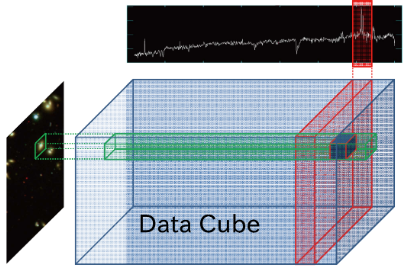
\includegraphics[width=0.45 \textwidth]{images/cube}
		\caption{The schematic illustration of a data cube of ALMA, with two spatial dimensions and a frequency or wavelength one \citep{eguchi_superluminal_2013}.}
		\label{fig:data_cube}
	\end{center}
\end{figure}

\section{Background} \label{sec:background}

% (1 Page)

\begin{comment}
    Spectroscopy
    - What is spectroscopy
    - What is an emission line
    - What an emission line allows to know
    - Common patterns in spectroscopy

    Sparse Coding
    - Global definition
    - Signal Applications
    - Dictionary
    - Mathematical Formulation: Equation and parameters
    - Approx Resolution of the Formulation
    - Type of Dictionaries: Defined and Learned
    - Applications to Images and De-noising

    Link between Spectroscopy and Sparse Coding
    - Variability Factors in Spectroscopy
    - High Dimensionality and Co-linearity
    - Sparse Coding as solution
    - Tools used (package)
\end{comment}


% Spectroscopy
\subsection{Spectroscopy}
% What is spectroscopy
Spectroscopy is a technique that enables the analysis of interaction between matter and light \citep{smith_mr_sp_2005}.
This analysis provides information on chemical structures and physical forms that can be used to identify substances from the characteristic spectral patterns.
These patterns appear as light intensity peaks observed along the spectra, known as emission lines \citep{struve_fundamentals_1989}.
% What is an emission line
Each line has a different frequency depending on the molecule and energy level associated to it \citep{smith_mr_sp_2005}.

% What an emission line allows to know
Detection of emission lines and subsequent association with a molecule's isotope allow to know stellar objects's molecular structure.
The combination of emission lines for each object generates an unique fingerprint.
This allows to identify similar objects observing the similarities between observed spectra and theoretical known behavior of molecules \citep{howley_effect_2005}.

% Factors that make this problem non-trivial
A traditional process to identify lines consist on mapping observed frequencies to theoretical ones.
Unfortunately, observed and theoretical intensities do not coincide. For instance,
two spectral lines that are close in the frequency space are hard to dissociate, mainly because they appear
as lines with double peaks or blended into one single line \citep{cernicharo_detection_2013, smith_molecular_2015}.

% Common patterns in spectroscopy
Internal factors such as the temperature of objects, travel speed, type of astronomical object and its belonging to interstellar or intergalactic space \citep{sembach_far_2001} cause variability in the observed spectra.
However, the presence of lines within objects of similar composition are in general similar.
Lines present from the same isotope at different state energy levels, and thus, different frequencies, reinforces the hypothesis that an isotope is present.
This analysis of the presence and co-presence of spectral lines from the same isotope is known as rotational spectroscopy \citep{schilke_line_2001}.

There exists a relationships among intensity lines when homogeneous temperature and origin are assumed, i. e., local thermodynamic equilibrium (LTE) exists.
For different stellar objects, and for different spectra measured within the same object, intensities of spectral lines with the same frequency may vary \citep{madden_classification_2005}.
However, relationships between intensities of rotational sequences for the same object should be consistent but not necessarily linear \citep{nummelin_three-position_2000, smith_molecular_2015}, as can be seen in figure \ref{fig:spectral_lines}.

Noise and lack of sensitivity in the measurements can either modify the frequency of a spectral line or produce false positives \citep{nummelin_three-position_1998}.
This makes mandatory to involve astronomers to perform the identifications \citep{schilke_line_2001}.

\begin{figure}[H]
   	\begin{center}
   		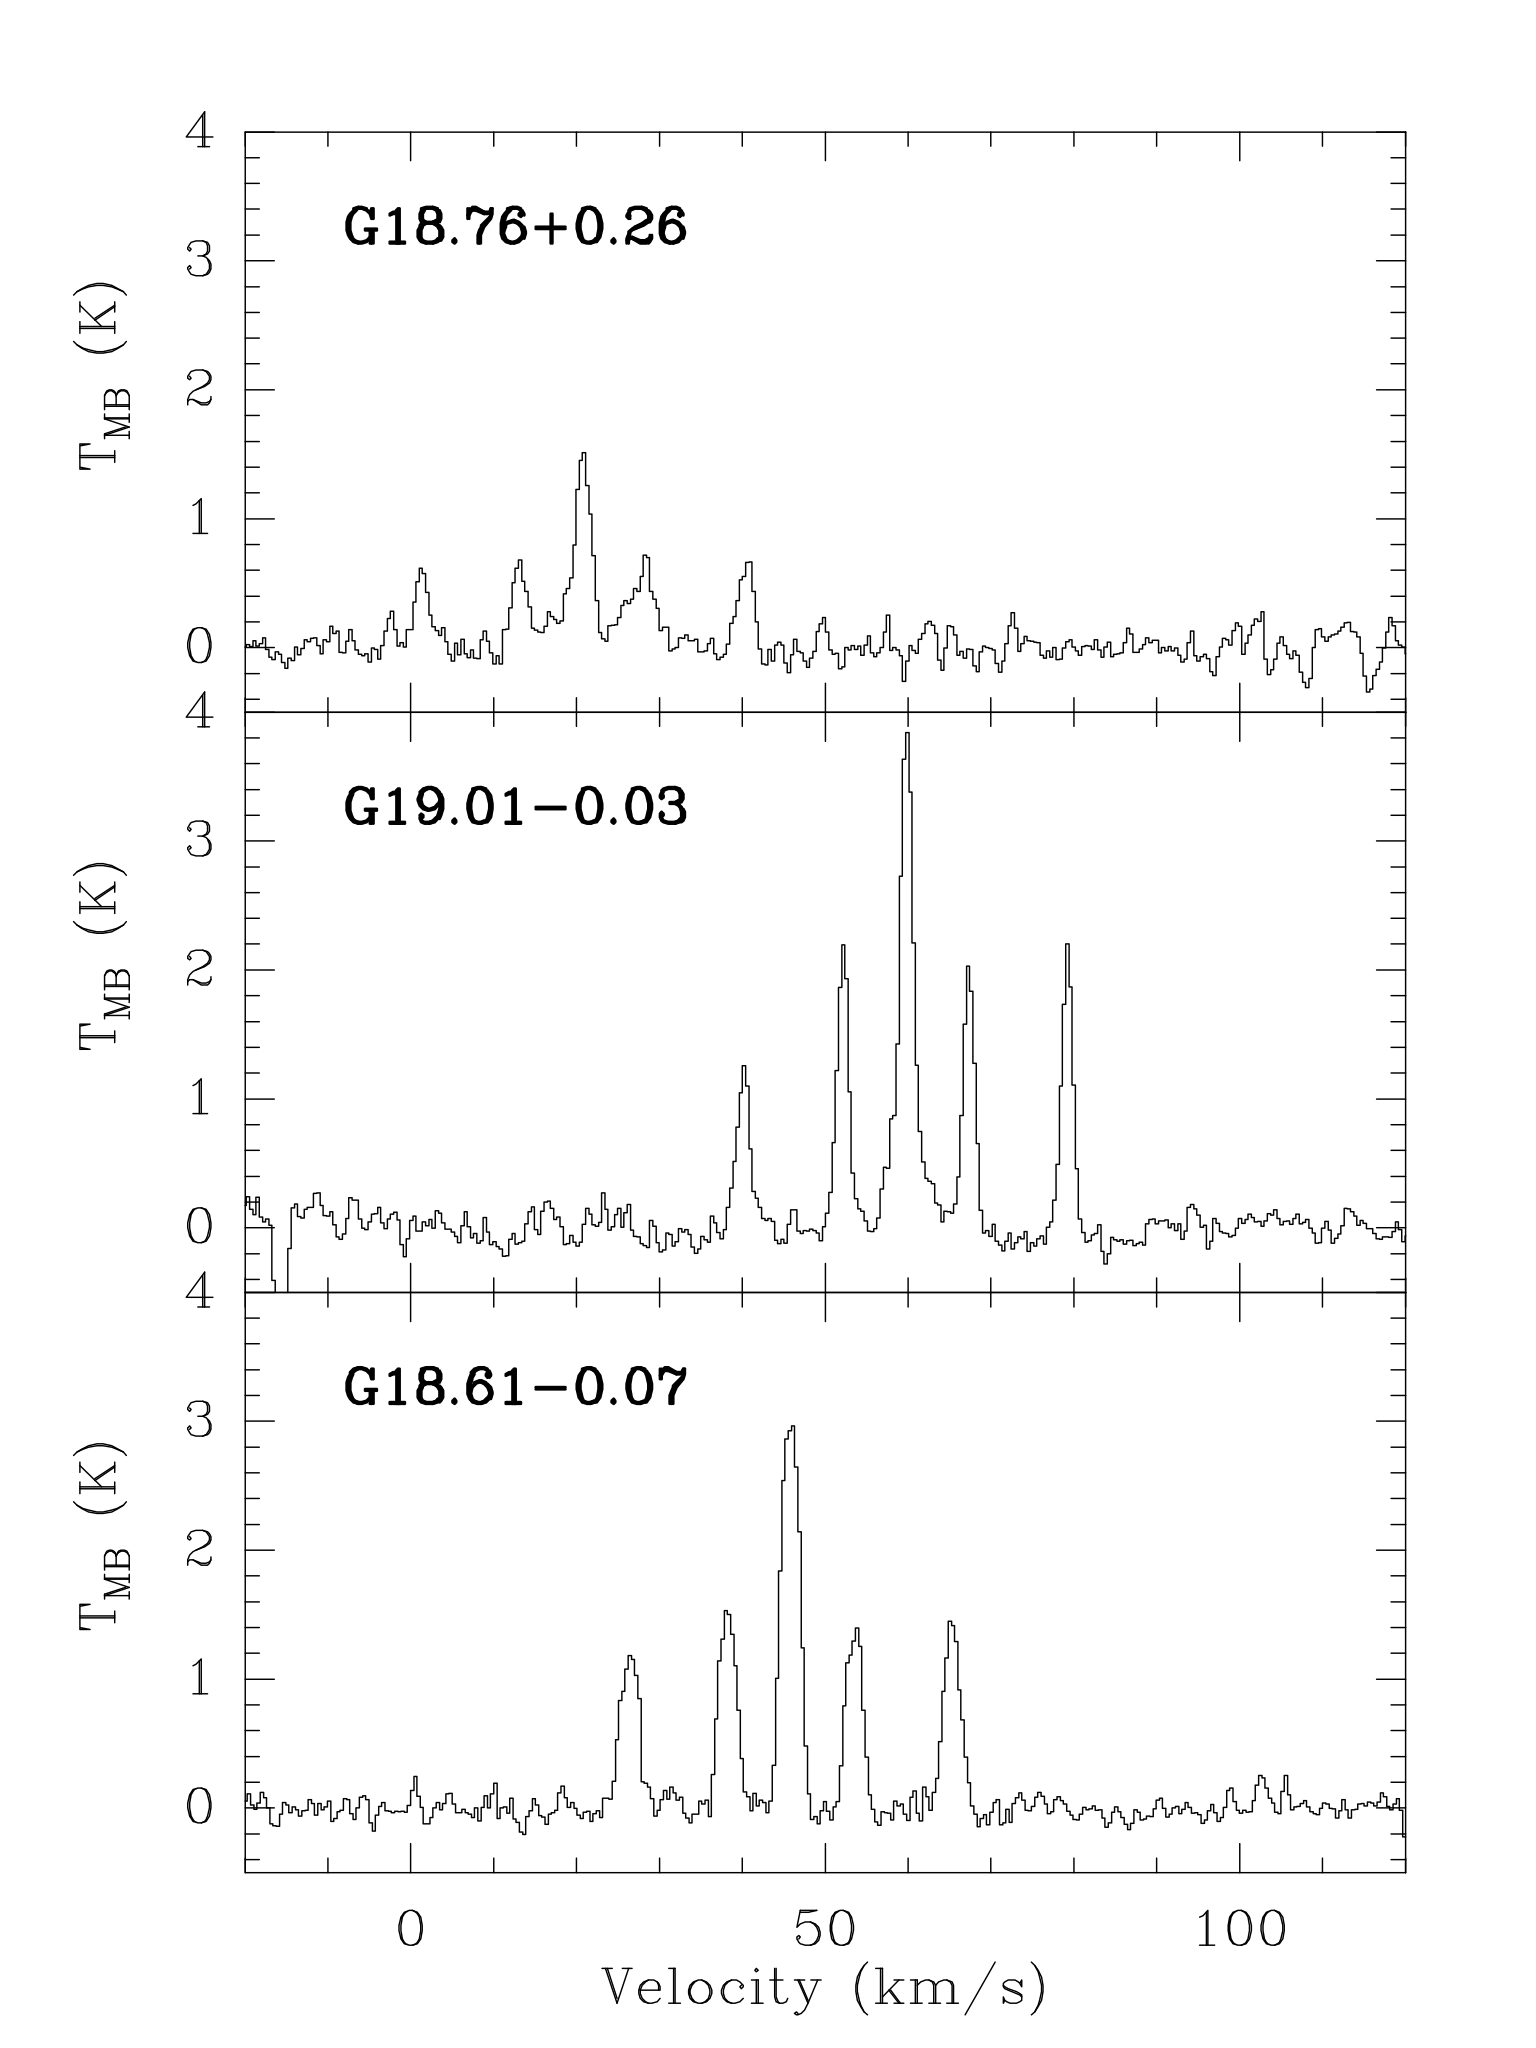
\includegraphics[width=0.40\textwidth]{images/spectral_lines}
   		\caption{Example spectra in a NH$_3$ transition for three sources.
   			We can see variations in velocity and intensity besides the similar structure \citep{schuller_atlasgal_2009}.}
   		\label{fig:spectral_lines}
   	\end{center}

\end{figure}

% Sparse Coding
\subsection{Sparse coding}
% Global Definition
Sparse coding consist in modelling signals through linear combinations of basis vectors under sparsity constraints,
in order to have a sparse representation of input signals \citep{mairal_online_2009, bristow_fast_2013}.
%
% Signal Applications
Sparse coding aims to represent or recover a signal through a reconstruction procedure.
We can divide this process in two main steps:
i) find a set of fundamental components able to represent any possible signal by linearly combining the components;
ii) for a given signal, determine the coefficients of the linear combination that minimize the difference between the signal and the linear combination of the components.
% Dictionary
Fundamental components set is known as \textit{dictionary}, where each component is called a \textit{word} \citep{mairal_online_2009}.
%
% Mathematical Formulation: Equation and parameters

Formally, let $s = [s_1, s_2, \ldots, s_n]$ be a given signal, where $s_i \in [0, 1] \; \forall i \in [1, \ldots, n]$.
Let $D = \{ w_1, w_2, \ldots, w_d \}$ be the dictionary, where $w_i = [w_{i1}, \ldots, w_{in} ]$ and $w_{ik} \in [0,1] \; \forall i \in [1, \ldots, d] \; \forall k \in [1, \ldots, n]$. Let $\alpha = [ \alpha_1, \ldots,  \alpha_d]$
be the set of coefficients such that $s = \sum_{i=1}^{d} \alpha_i \; w_i $.
Equation \ref{eq:sparse_coding} corresponds to the optimization problem that has to be solved in order to determine the sparse coding coefficients.

\begin{equation}
	\label{eq:sparse_coding}
    \begin{aligned}
		\text{Minimize}
		& _{\alpha} ||s- \sum_{i=1}^{d} \alpha_i \; w_i  ||_2^2  \\
		\text{Subject to: }
		& ||\alpha||_1 \leq \lambda \\
		& \alpha \geq 0 \\
	\end{aligned}
\end{equation}
where $||()||_k$ is the L-$k$ norm, and $\lambda$ is sparsity-inducing constant.

The solution to this problem is known as positive basis pursuit \citep{chen_atomic_2001} or positive lasso regression \citep{efron_least_2004}.
The optimization solution solved in closed form is very expensive in terms of processing \citep{mairal_online_2009}, instead,
we use the iterative algorithm presented in \citet{turlach_simultaneous_2005, mairal_optimization_2013}.

There are two constraints applied to alpha values: i) the lambda sparsity-inducing constraint allows the algorithm to select a convenient set of basis vectors so that the number of non-zero values minimized;  ii) the positive formulation of the problem allow us to give a meaningful use to the found set of alpha values; both are detailed in section \ref{sec:algorithm}. 

% Type of Dictionaries: Defined and Learned
In sparse coding, there exist two types of possible dictionaries to create the basis vector set:
i) Previously defined one, where a set is selected accord to the nature of signal domain.
ii) Automatically learned one, where methods such as clustering or another generalization searching are used \citep{mairal_online_2009}.
For wavelength domains, predefined dictionaries give satisfactory results \citep{mallat2009}.

% Applications to Images and De-noising
%Sparse Coding is a well known technique in visualization applications.
%Example of this are image classification, de-noising and image reconstruction \citep{mairal_online_2009}.
%In these cases, words are automatically learned as patches from image sets.
%Then, the most representatives patches are selected to replicate as much images as possible from the learned image sets.
% Tools used (package)
%The software used in this work is the Python library SPAMS available for Matlab and R as well \footnote{\url{http://spams-devel.gforge.inria.fr/}}. \citep{mairal_online_2009,mairal_online_2009_2}


\section{Related work} \label{sec:related_work}

% Present Tense
\begin{comment}
    - What is currently being done
    - Manual Process Problems
    - Factors that make this problem non-trivial
    - Semi-Automatic Method
    - Ramadan Spectroscopy
    - Physics Models
    - Utility of another approach (this approach)
\end{comment}

% What is currently being done
In the last years, detection of spectral lines has been following traditional methods, limited to manual analysis of data.
This analysis primarily involves the estimation of frequencies associated to peaks in spectra, together with the mapping of those peaks
to theoretical frequencies.
After determining the presence of the lines at different frequencies, they associate those lines to certain isotope energy states.
This non-automated process lacks of scalability, making impossible to apply this method for large databases \citep{schilke_line_2001}.

Spectra classification is found in other areas such as classification of substances, determination of raw material purity or even detection of skin cancer \citep{sigurdsson_detection_2004}.
Supervised machine learning classifiers have been proposed to separate different types of substances within spectra \citep{howley_effect_2005}, but they are not designed to identify individual lines.

Several methods specialize in the individual detection of lines along the spectra.
For example, EMILI software identifies spectral lines considering three features:
i) wavelength agreement with observed line, 
ii) expected flux from relative computed intensities and
iii) co-presence of other confirming lines.
It assign numerical values to each criteria and calculates a score with them, both for observed lines and candidate theoretical lines.
Then, probabilities are calculated for each candidate line.
The near its score, the higher its probability \citep{sharpee_introducing_2003}.

% Ajustar funciones para modelar el ancho optico de las lineas es una tecnica muy comun de uso extendido y actual.
To fit functions to shape the optical depth of lines is a very common technique still widely used.
% Funciones Gaussianas y Top-Hat pueden ser ajustadas a través de la estimación de tanto el fwmh como la intensidad de las lineas]
Gaussian functions \citep{fuller_thermal_1993, nummelin_three-position_2000} or top-hat functions \citep{smith_molecular_2015} are adjusted through the estimation of both the full width maximum height ($fwmh$) and peak intensities for line profiling.
% Un parametro de 'desplazamiento de la línea base residual' es determinado para diferenciar lineas del ruido de la señal.
Then, a residual baseline offset is set to differentiate lines from signal artifacts.

Tools that fits more complex functions to spectra are 
XCLASS \footnote{\url{https://www.astro.uni-koeln.de/projects/schilke/XCLASS}},
CASSIS \footnote{\url{http://cassis.cesr.fr}} and
WEEDS \footnote{\url{https://www.iram.fr/IRAMFR/GILDAS}}.
These tools fit different functions along the spectra to estimate several parameters of observed lines.
They build a line list fitting of all the transitions of an isotope through two steps:
i) the fit of the line, 
ii) the fit of the baseline.
For fitting of lines, CASSIS determines optimal parameter functions that allows to simultaneously fit all peaks along spectra. Gauss, Lorentz, Sinc and Voight are examples of functions for fitting lines. 
Then, in step ii), weaker lines are discarded fitting a baseline function, which can be sinusoidal or polynomial functions \citep{caux_cassis_2011,vastel_cassis_2015}

These tools make use of catalogs of spectral lines that contains the theoretical frequencies of all known lines for each isotope.
Those catalogs are publicly available, and are constructed by the data of
(JPL \footnote{\url{http://spec.jpl.nasa.gov}},
CDMS \footnote{\url{http://www.astro.uni-koeln.de/cdms}},
Toyama \footnote{\url{http://www.sci.u-toyama.ac.jp/phys/4ken/atla}}).
Unfortunately, a lot of human effort is needed just to identify spectral lines in this way as \citep{schilke_analysis_2011} states.

Furthermore, chemical and physical models takes into account the source structure through a modelling, using complex simulations to reproduce stars formation and later, spectral lines. These simulations involve two main steps:
i) 3D chemical models and 
ii) radioactive transfer models \citep{schilke_analysis_2011}.
In step i), the structure of object is modeled using molecular abundance, which is used either from provided values or from chemical models.
An example of programs to get molecular abundance is RATRAN \citep{hogerheijde_accelerated_2000}.
In step ii), the structure temperature of cores are estimated using Monte Carlo.
Both \textbf{radme-3d} \footnote{\url{http://www.ita.uni-heidelberg.de/~dullemond/software/radmc-3d/}}
and LIME \citep{brinch_lime_2010}
use this sampling simulation assuming LTE approximation.
The first estimates object temperature, while the latter receives it as a parameter.
An analysis of line shapes and temperature modeling allow to assign them to known isotope lines.

Regarding signal reconstruction models, approaches that compares observed spectra with synthetic modelling have been proposed in \citep{pequignot_deep_1996, walsh_deep_2003}.
These models have a rigorous treatment of blending and have the flexibility to deal with wavelength uncertainty from databases \citep{sharpee_introducing_2003}. 
Techniques described above are in general not scalable, do not rely on automatic processes or are based on complex theoretical underlying models. 


\begin{comment}
- Problem Formulation
	-- Physics Abstraction
	-- ALMA like Data
	-- Need of Synthetic Data
	-- Algorithm Input
	-- Algorithm Output
	
- Data Origin
    -- Splatalogue. What is it?
    -- Splatalogue. What allows to know?
    -- ASYDO. What is it?
    -- Simulation Features (and simplifications)
    -- First View to Predition Validation (We know the simulated lines present)
    -- ASYDO Parameters; Algorithm Parameters
    -- Redshift types
    -- Noise in each Band
    -- Line width
\end{comment}

% Data Origin
\section{Data} \label{sec:data_origin}
 
\subsection{Synthetic data}
% Need of Synthetic Data
% La solución que proponemos no depende de la quimica o fisica subyacente, por lo que es necesaria una cantidad suficiente de datos para encontrar patrones en la detección de líneas.
The solution proposed does not rely on underlying physics or chemistry, so it need enough data to find line-detection patterns.
At this time, available spectral data from ALMA is not enough, hence the use of synthetic data is necessary.

% Algorithm Input
% Synthetical data is generated through the simulation of data cubes with chemical components belonging to certain known group of isotopes.
% Algorithm Output
% The algorithm, only analyzing the spectra of this data cubes, gives a list with probability distribution of isotopes that could have generated the observed lines.
% With the simulated data, the actual lines that are present in the spectra can be known, so each prediction made by the classifier can be validated.

In the next section, the tools to get synthetic data are introduced and also, its use in this project.

% Splatalogue. What is it?
\subsection{Splatalogue. Catalogue of theoretical lines}
Splatalogue is the most up-to-date and complete spectral line database.
%
It consists in a catalog of experimental lines that gives a list of all known frequency for isotopes at their different known transitions states \citep{remijan_splatalogue:_2008}.
%
It aims to contain all known emission line data currently archived from labs all over the world - Jet Propulsion Laboratory (JPL), The Cologne Database for Molecular Spectroscopy (CDMS) \citep{muller_cologne_2005}, Lovas National Institute of Standards and Technology (NIST), among others sources \citep{remijan_splatalogue_2010}.

% Splatalogue. What allows to know?
Also, it allows to filter and search for spectral lines by isotope and wavelength ranges.
This tool is important for this work, since it is used to create the dictionary.

% ASYDO. What is it?
\subsection{ASYDO. Synthetic data}

The Astronomical Synthetic Data Observations (ASYDO) package \footnote{\url{https://github.com/ChileanVirtualObservatory/ASYDO}} is used to simulate ALMA-like data.
The simulation generates a training set to develop and test identification accuracy.
    
\begin{figure}
	\begin{center}
		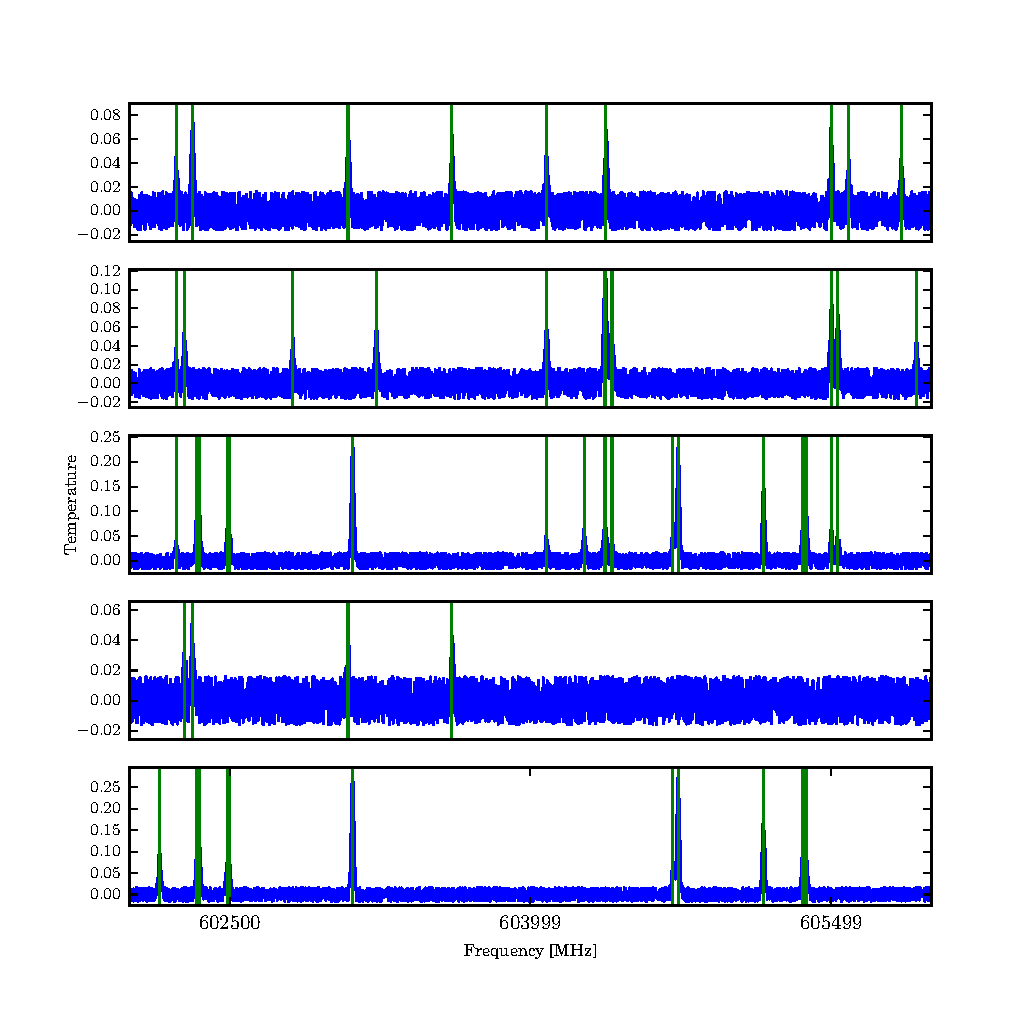
\includegraphics[width=0.45\textwidth]{images/overview}
		\caption{Example of ASYDO simulated spectra. Green vertical lines correspond to theoretical isotope lines used for the simulation.}
	\end{center}
	\label{fig:overview}
\end{figure}
    
% ASYDO Parameters
ASYDO can create fits files containing simulated hypothetical stellar objects using the next parameters:
%
\begin{easylist}[itemize]
& \textbf{Isolist}     : subset isotope list to generate a cube
& \textbf{Parameters}
&& \textbf{freq}         : spectral center (MHz)
&& \textbf{spe\_res}     : spectral resolution (MHz)
&& \textbf{spe\_bw}      : spectral bandwidth (MHz)
&& \textbf{(fwhm}, \boldmath{$\alpha$} \textbf{-skew}): skew-normal distribution parameters (MHz, parameter)
\end{easylist}

Skew-normal function gives form to spectral lines, in which $fwhm$ is full width at half maximum, and $\alpha-skew$ is its kurtosis parameter.
If $\alpha-skew = 0$, it degenerates to a Gaussian function, if $\alpha-skew < 0$, it is left-biased and $\alpha-skew > 0$, a right bias.

% Redshift types
We assume object movement redshift as known and corrected. 
A previous step is necessary to identify a set of stronger lines in the spectra and determine velocity shift \cite{sharpee_introducing_2003}.
Eliminating general redshift just left two error margins for observed frequencies: noise and internal redshift given by rotation and internal movements.

% Noise in each Band
Each band has different noise because of both radio-telescope sensitivity at each band, and nature of spectra signals at different wavelengths.

% Line width
The width of each line depends on skew-normal parameter $fwhm$.
For testing purposes, we modified the width in a 4 MHz range with a modification of ASYDO, incorporating this randomness to use different width for each spectral line.
The parameters we use for simulations are: both \textbf{alpha} and \textbf{delta} as 0 $degrees$, \textbf{spe\_res} of 1 $MHz$, \textbf{spe\_bw} as 4000 $MHz$ and \textbf{(fwhm}, \boldmath{$\alpha$} \textbf{-skew}) as $(8, 0)$.



\begin{comment}
-- Algorithm
 - 1. Pre-processing
	i) Raw data
	
	ii) Filtering, Normalization
	-- Savitzky-Golay Filter and Normalization

	iii) Delta Dirac Functions
	  -- Dictionary Generation
	  -- Dictionary as Dirac Deltas Functions
	  -- Hyperfine Lines
	  -- Independent words
	
	iv) Detection of Lines
	  -- Detection of Candidate Lines: Local Maxima and Minima
	  -- Threshold Detection
	  -- Gaussian Subtraction
	
	v) Recalibration
	Recalibration. Need of Exact Match for Sparse Coding
		a) Exponential Kernel
			Flexibility of the Solution: Gaussian Kernel
		b) Intensity Weight
			Including temperature: Weight

 - 2. Classification
	  -- Lambda Parameter
	  -- Alpha Constraints
	  -- Pseudo-Code
	  
-- Training Set/Tests
	  -- Specifications of Data Cubes
	  -- Different Bands and Variable/Fixed Widths
	  -- Modified Confusion Matrix
\end{comment}

% Algorithm
\section{Algorithm} \label{sec:algorithm}

\begin{figure*}
	\begin{center}
		% 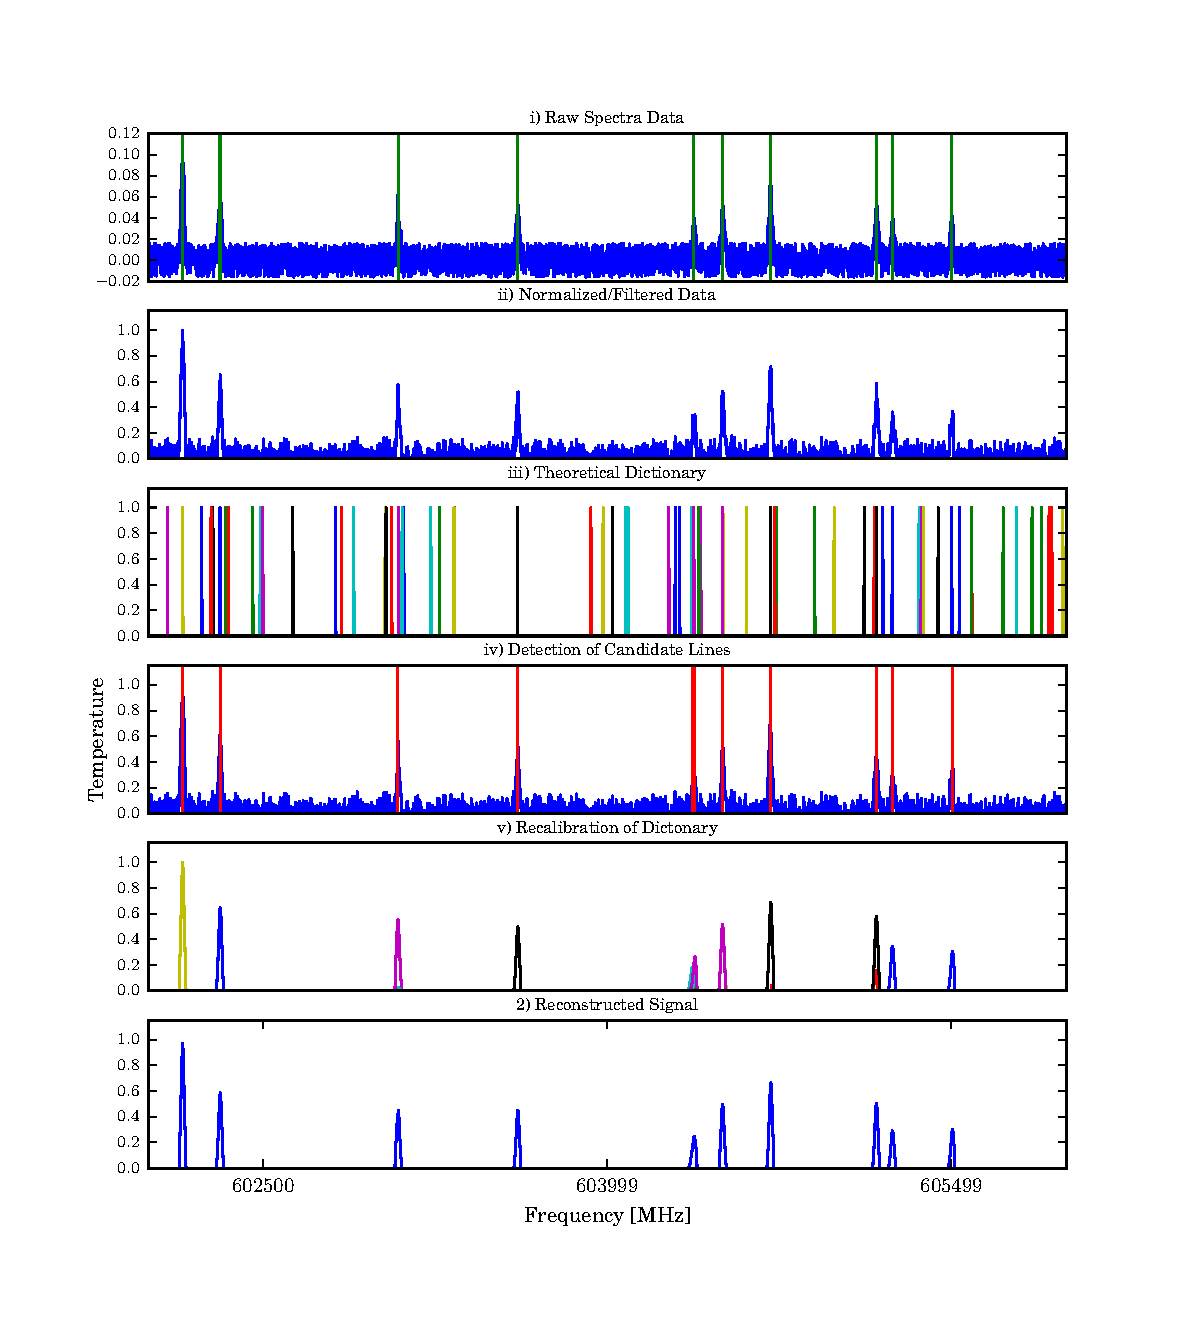
\includegraphics[width=\textwidth]{images/process}
		\label{fig:process}
		\subfigure[]{
			\label{fig:a}
			\clipbox*{0 {.786\height} {1\width} {.9055\height} }{%
				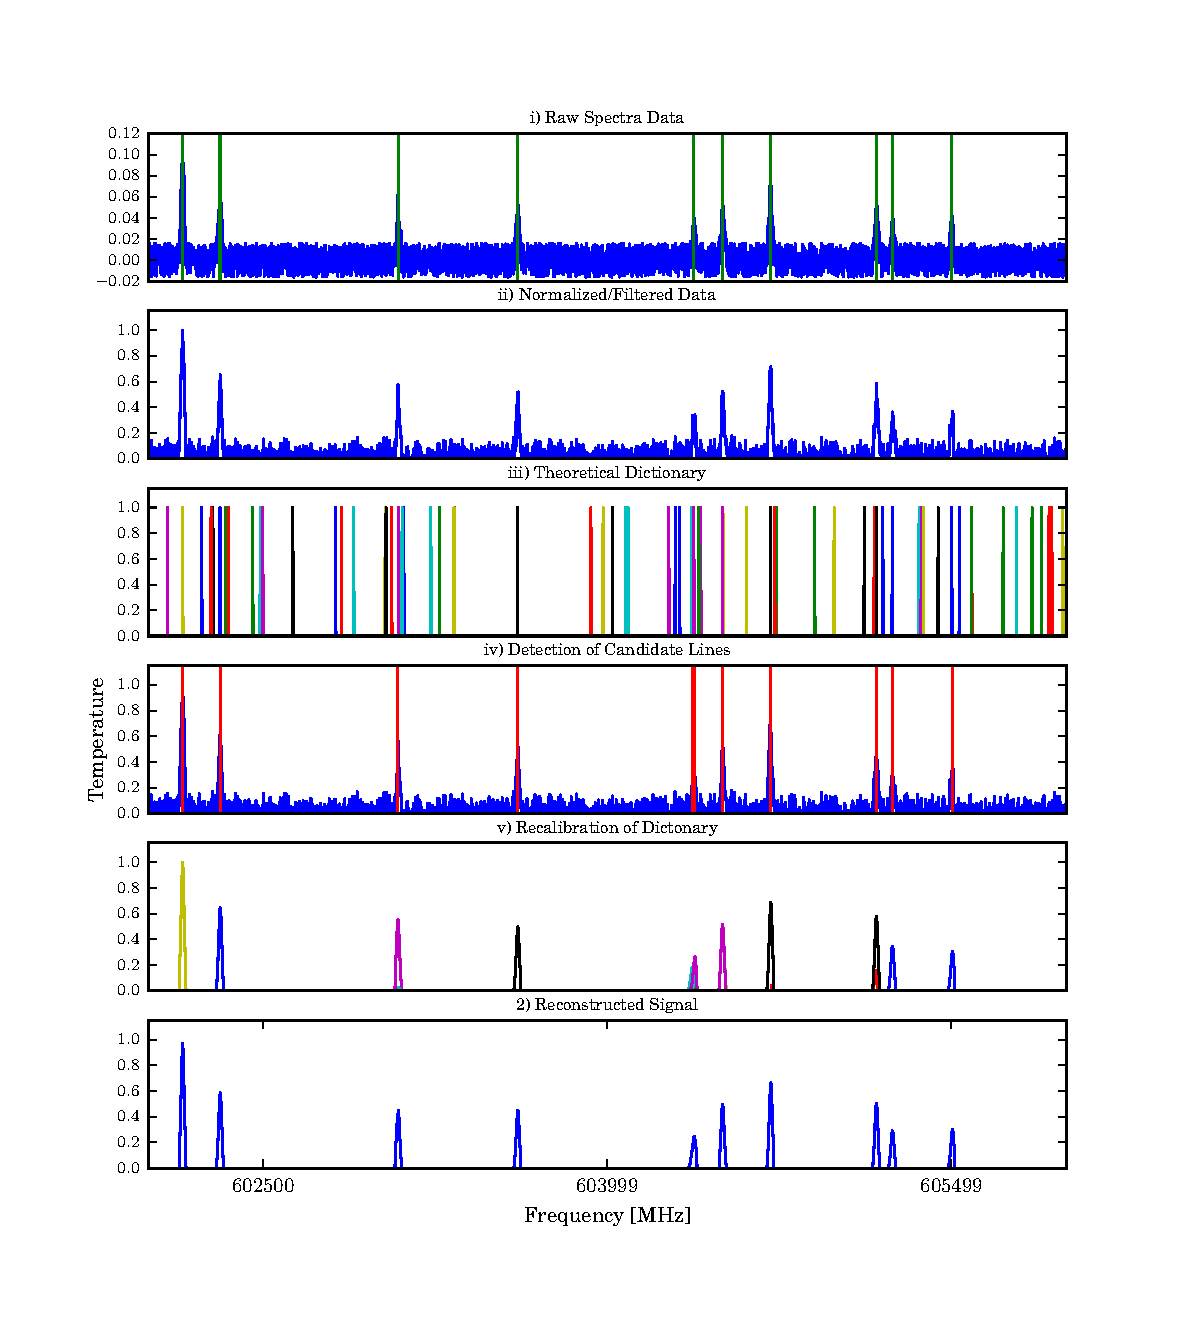
\includegraphics[width=\textwidth,height=450px]{images/process}%
			}%
		}
		\subfigure[]{
			\label{fig:b}
			\clipbox*{0 {.653\height} {1\width} {.770\height} }{%
				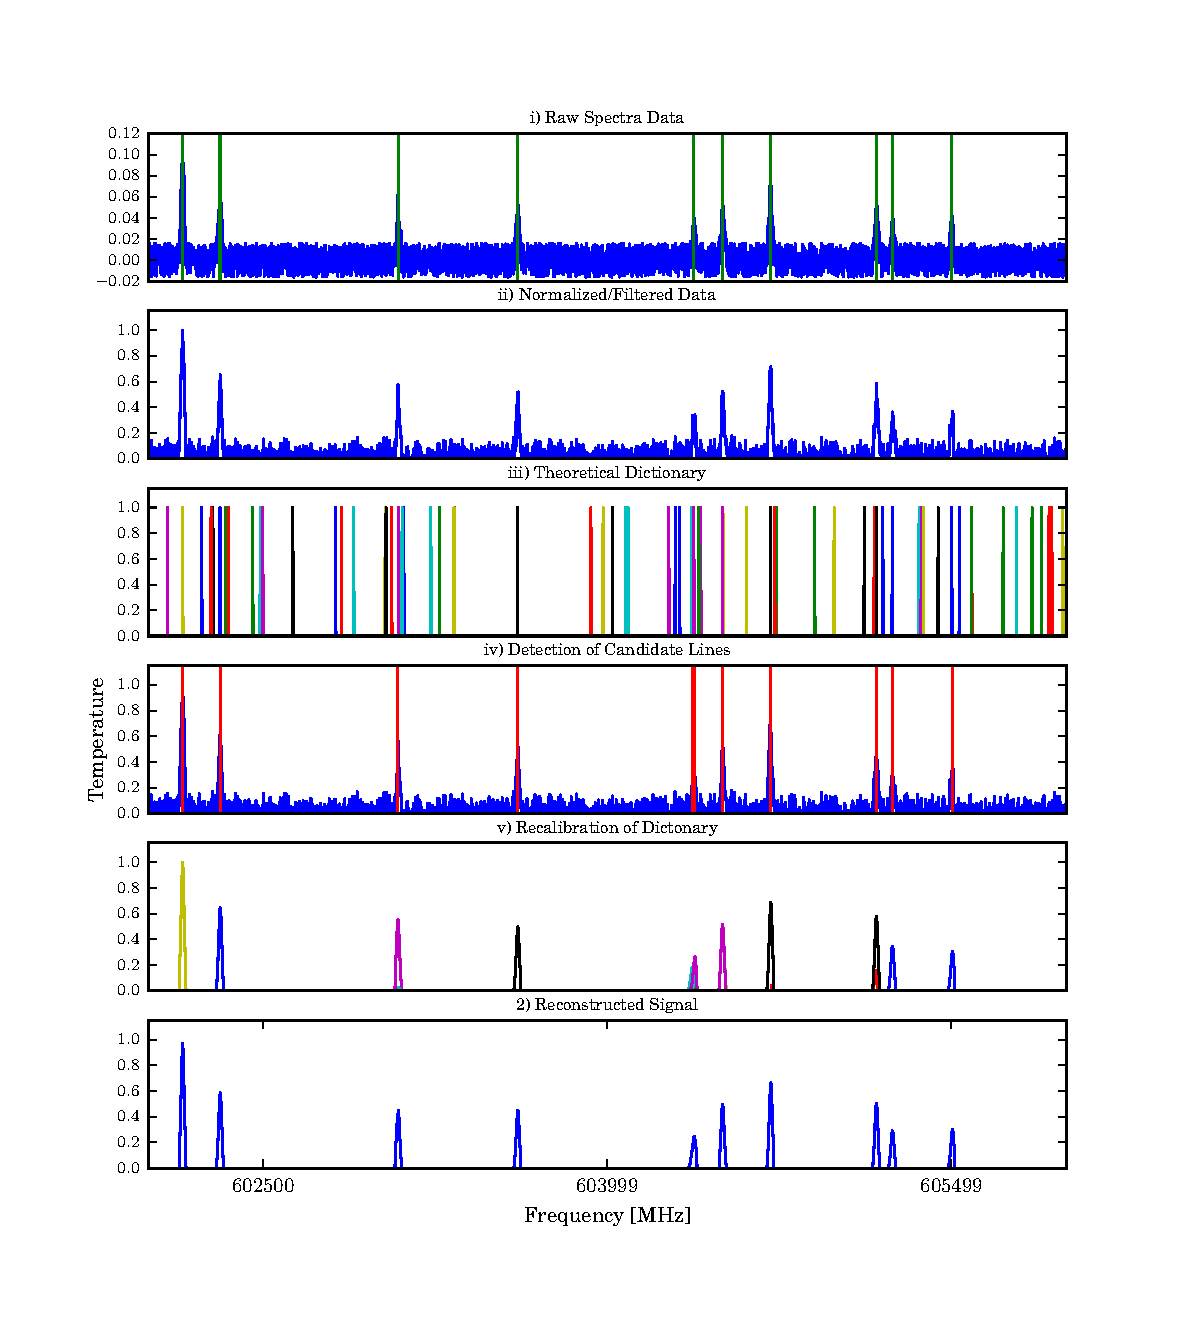
\includegraphics[width=\textwidth,height=450px]{images/process}%
			}%
		}
		\subfigure[]{
			\label{fig:c}
			\clipbox*{0 {.520\height} {1\width} {.640\height} }{%
				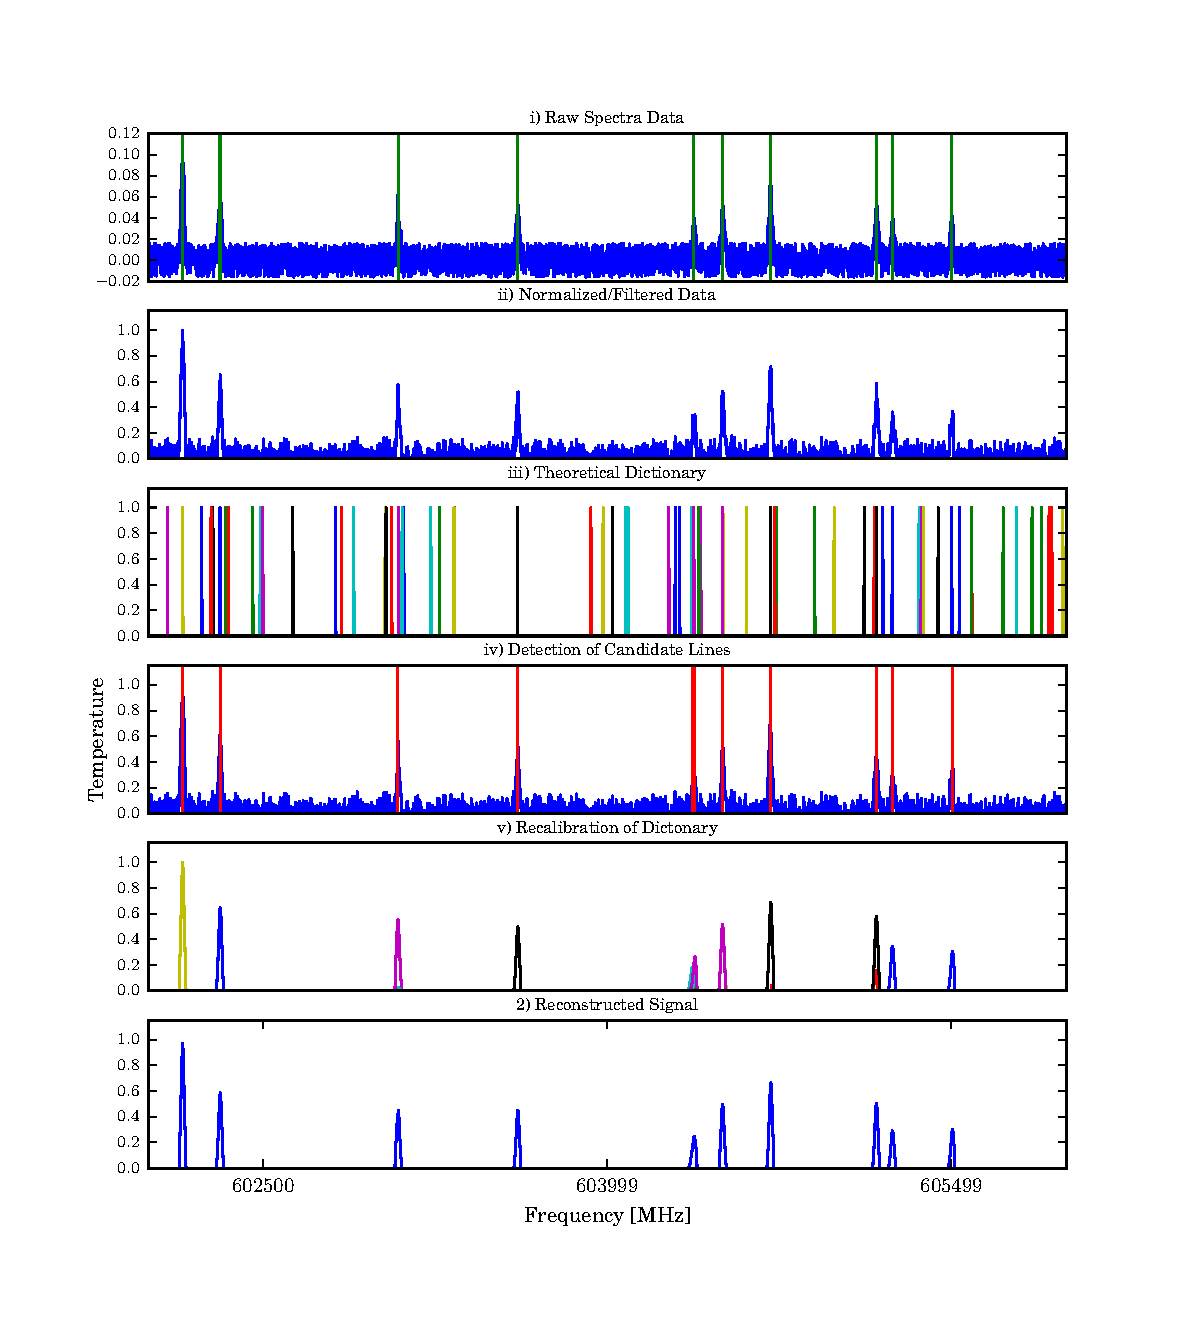
\includegraphics[width=\textwidth,height=450px]{images/process}%
			}%
		}
		\par\medskip
		\subfigure[]{
			\label{fig:d}
			\clipbox*{0 {.387\height} {1\width} {.505\height} }{%
				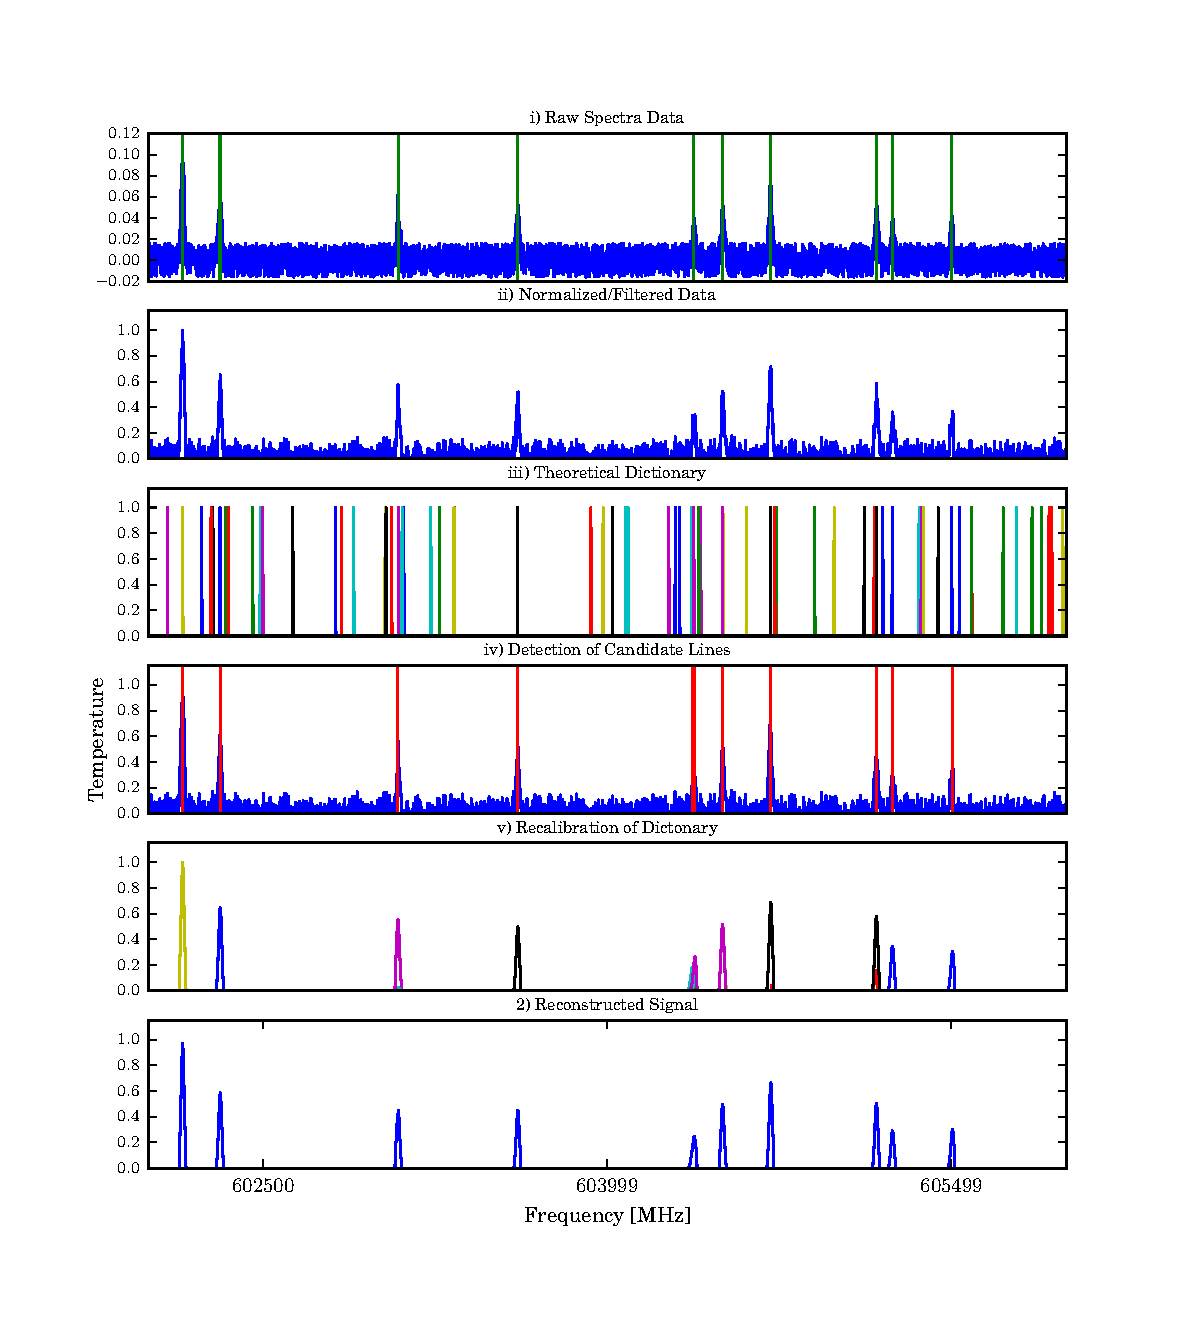
\includegraphics[width=\textwidth,height=450px]{images/process}%
			}%
		}
		\subfigure[]{
			\label{fig:e}
			\clipbox*{0 {.254\height} {1\width} {.370\height} }{%
				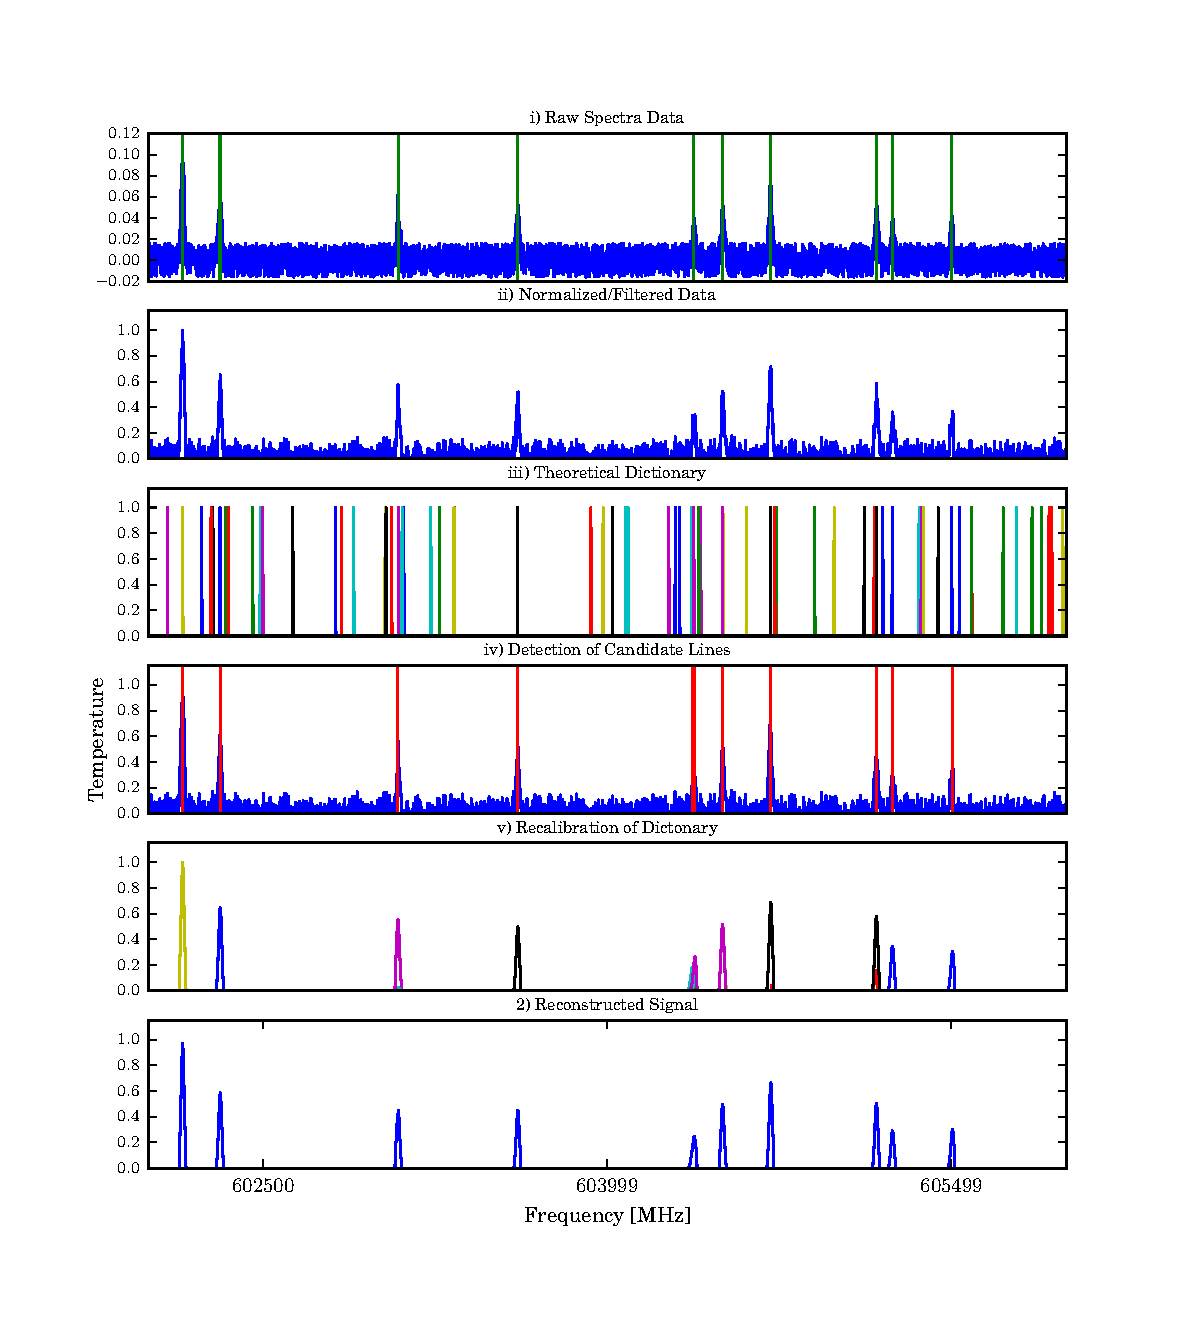
\includegraphics[width=\textwidth,height=450px]{images/process}%
			}%
		}
		\subfigure[]{
			\label{fig:f}
			\clipbox*{0 {.08\height} {1\width} {.240\height} }{%
				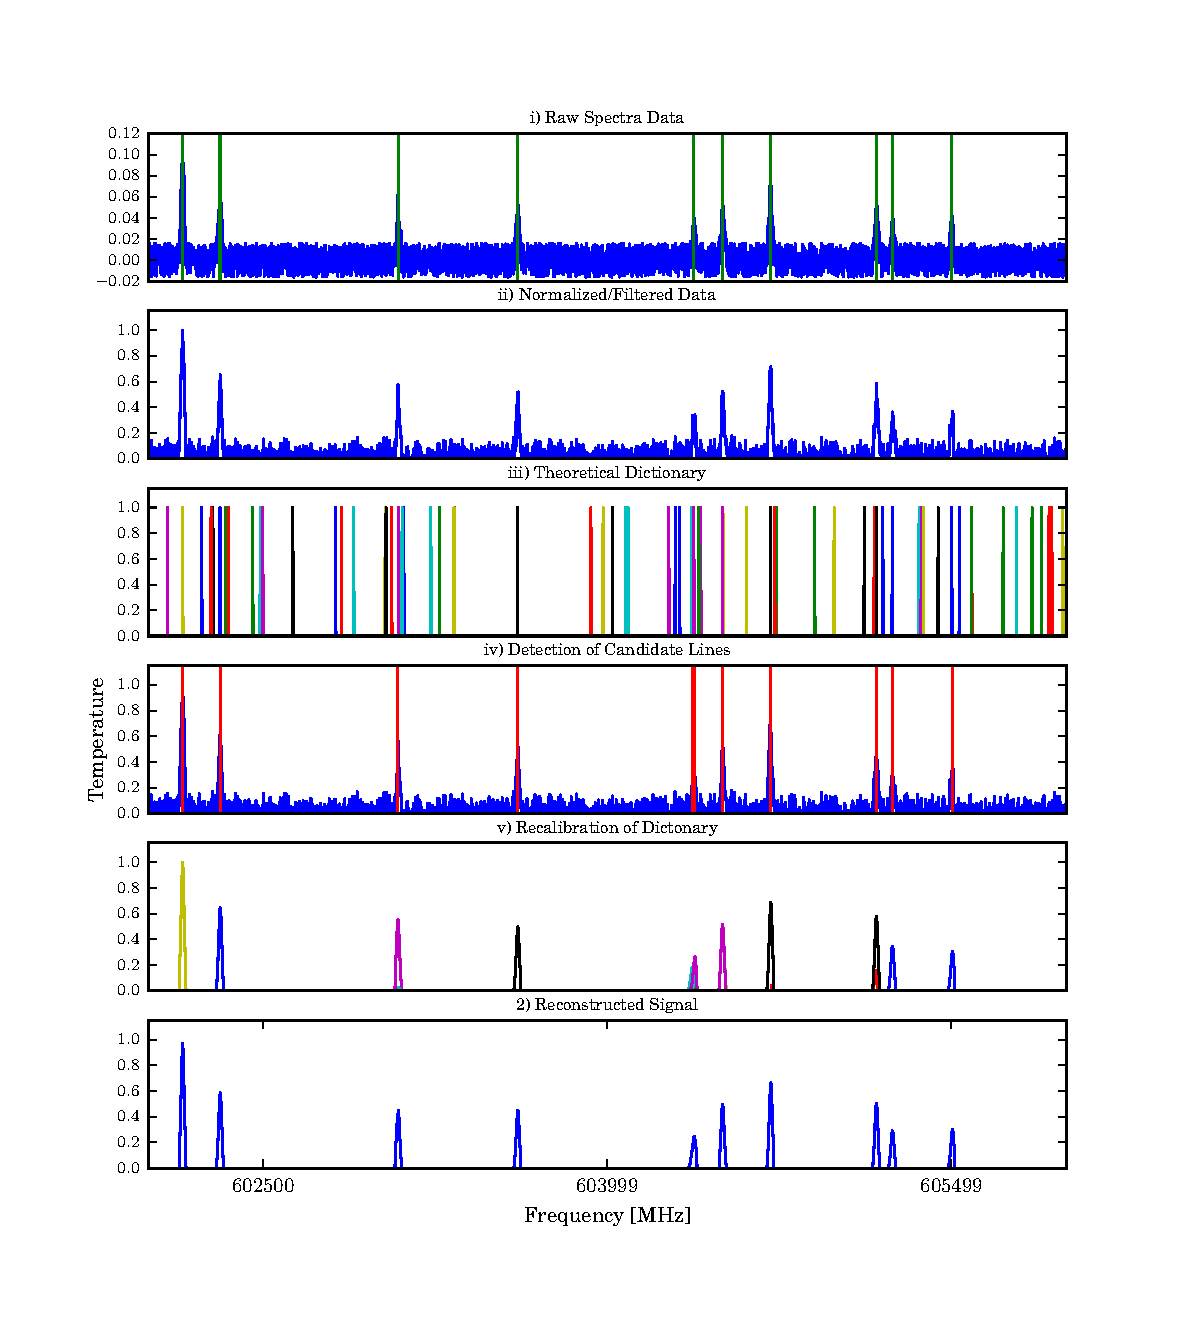
\includegraphics[width=\textwidth,height=450px]{images/process}%
			}%
		}
		\caption{Spectra example though the whole process. Each step: 1. Pre-processing: (a) Read raw data cube, (b) Filter and normalize, (c) Determine dictionary, (d) Detected candidate lines, (e) Recalibrate the dictionary. 2. (f) Reconstruction of the signal.}
	\end{center}
\end{figure*}

Our algorithm has two main steps:
i) spectra pre-processing, which also involves the creation and recalibration of the dictionary, covered in section \ref{sec:preprocessing}.
ii) optimization of equation \ref{eq:sparse_coding}, which allow us later to predict emission lines present along the spectra, viewed at detail in section \ref{sec:prediction}.
An overview of the process is illustrated in figure \ref{fig:process}.

% Pre-processing
\subsection{Pre-processing}  \label{sec:preprocessing}

At first, a dimensional pixel from a data cube is selected to analyze its wavelength range, as shown in figure \ref{fig:a}.
Then, a normalization and filtering of spectra is performed.
Savitzky-Golay filter is applied to reduce white noise influence along the signal\citep{howley_effect_2005}.
Normalization does not have any effects in the sparse coding solution, however, it is applied for convenient purposes, as we will explain later.
Figure \ref{fig:b} illustrates the output after the preprocessing step.

% Dictionary as Dirac Deltas Functions
\subsubsection{Delta Dirac function}
In this stage, we perform the following steps: 
i) select all theoretical lines for all isotopes present in range of measurement.
ii) create delta Dirac vectors for each theoretical line previously selected.
Delta direct functions allow to determine a representative and meaningful dictionary for this problem.
One word is defined for each theoretical frequency known in spectra wavelength range.
This formulation allows to represent each theoretical frequency range with a specific word in the dictionary.

Let $D = \{ w_1, w_2, \ldots, w_d \}$ be the dictionary, where $w_i = [w_{i1}, \ldots, w_{in} ]$ and $w_{ik} \in [0,1] \; \forall i \in [1, \ldots, d] \; \forall k \in [1, \ldots, n]$.
Let $F = \{ f_1, f_2, \ldots, f_n \}$ be the set of frequencies at the range of measure.
The value of each element of $w_i$ is given by the function:

\begin{equation}
	 w_{in} =
	 \begin{cases}
	  1,& \text{if } f_i \text{ is the theoretical frequency of isotope } i\\
	  0,              & \text{otherwise}
	 \end{cases}
	 \label{eq:delta_dirac}
\end{equation}

Figure \ref{fig:c} lists all the theoretical frequencies combined along the spectra in range of measure.

Hyperfine lines are a particular case, in which two close theoretical lines that belong to same isotope are present. In general they are both present as one wider line (see figure \ref{fig:87_77_13C3}).

\begin{figure}[H]
	\begin{center}
		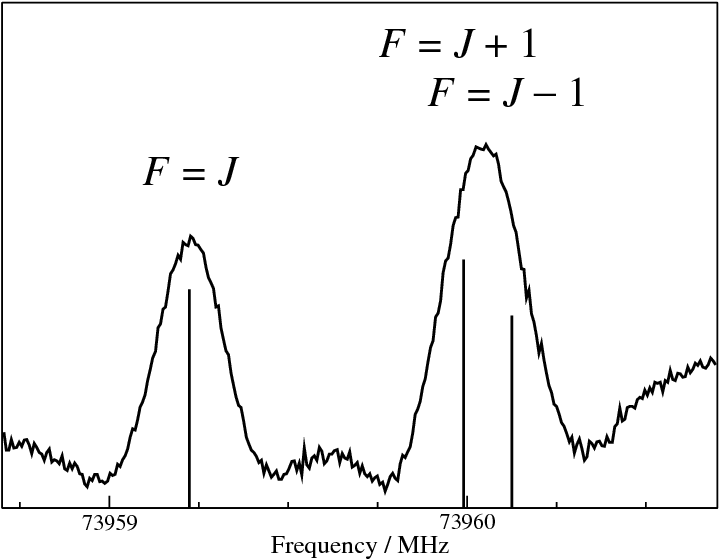
\includegraphics[width=0.35\textwidth]{images/87-77_13C3}
		\caption{Rotational spectrum of vinyl cyanide transition of H$_2^{13}$C=CH−C≡N showing hyperfine unseparable structures \citep{muller_rotational_2008}.}
		\label{fig:87_77_13C3}
	\end{center}
\end{figure}

To deal with hyperfine lines, we combine their delta Dirac functions and merge them into a single word.
Sensitivity of data determines when two hyperfine lines should merge as one.
As we use 1 MHz for sensitivity, two words are merged if they are closer that 1 MHz and belong to the same isotope.

A problem with the use of Dirac Delta functions is that observed lines must be at the precise observed frequencies to be used.
If a difference between a delta Dirac function and its observed candidate line exists, it is impossible for the sparse coding optimization to use the theoretical word to reconstruct the shifted observed frequency.
This makes necessary to adjust the previous words, so that a soft matching can be possible.
If a word is not at the exact frequency than a candidate line's frequency, but near it, the word still can be used, but with a loss of confidence.

Two steps are necessary to make this adjustment to the dictionary: 
i) detect all the candidate lines along the observed spectra, 
ii) expand each word in the recalibration step.

% Detection of Candidate Lines: Local Maxima and Minima
\subsubsection{Candidate emission lines}
We use an heuristic to pre-define frequency ranges at which further steps evaluate the presence or non-presence of emission lines.
A peak detection function is ran to select these ranges associated to possible lines along the spectra. We call these ranges candidate emission lines.

% Threshold Detection
We make use of a threshold given by the 3-$\sigma$ criterion.
An empty pixel is selected from a spectra of the data cube in which the observed object is not present, so that just background and noise is observable.
Then, we compute the mean and standard deviation of the noise.
With this, we search for intensity differences between each consecutive pair of frequencies, and when the difference between the temperature of a frequency and the previous temperature is higher that the threshold, the frequency from higher temperature is saved as candidate line.

% Gaussian Subtraction
Following this idea, an iterative process is performed.
All the peaks are detected from the original spectra and the frequency of the higher intensity is saved as a candidate emission line.
Then, a Gaussian function is fitted at the detected frequency and subtracted from the signal. The process is repeated until the higher intensity of the detected peaks is less than the  3-$\sigma$ threshold.
At the end of the process, a list of candidate lines is determined, as can be seen in figure \ref{fig:d}.

% Recalibration. Need of Exact Match for Sparse Coding
\subsubsection{Recalibration}

% Flexibility of the Solution: Gaussian Kernel
At the end of pre-processing step, the dictionary passes for a step of recalibration, where each word is expanded to a range from the initial Dirac delta function.
We use an exponential kernel function that assign values to each word depending on the distance between theoretical frequencies of the words and their nearest candidate lines.
Word's expansion allows to associate probabilities to matches, which are also used to combine several words at certain frequencies and to replicate blended lines.

In recalibration step, we introduce the use of candidate line's temperature to weight words according to the intensity of the nearest candidate lines.
This reflects that smaller candidate lines are less probable to be emission lines as they get closer in intensity to the threshold.
The final value of a word is given by equation \ref{eq:expansion}.

Let $s = [s_1, s_2, \ldots, s_n]$ be a normalized signal, where $s_i \in [0, 1] \; \forall i \in [1, \ldots, n]$.
Let $D = \{ w_1, w_2, \ldots, w_d \}$ be the dictionary, where $w_i = [w_{i1}, \ldots, w_{in} ]$ and $w_{ik} \in [0,1] \; \forall i \in [1, \ldots, d] \; \forall k \in [1, \ldots, n]$.
Let $F = \{ f_1, f_2, \ldots, f_n \}$ be the set of frequencies at the range of measure. 
Function $c(f)$ is defined as $c(f_i) = s_i, \forall i \in [1, \ldots, n]$, i. e., signal's intensity at frequency $f_i$.
$g$ is defined in \ref{eq:closer_candidate} as the closer candidate line's frequency to a given frequency $f_i$, such as for a word $w_{ki}$:

\begin{equation}
	\label{eq:closer_candidate}
	\begin{aligned}
		\text{$ g $}
		= 
		\text{argmin}
		& _{f} ||f_i - f|| \\
	\end{aligned}
\end{equation}

and a word's expansion is given by equation \ref{eq:expansion}
\begin{equation}
	\begin{aligned}
	\text{$ w_{ki} $}
	= \text{$ c{(g)} $} \cdot \frac{1}{\sqrt{2\pi\sigma}}e^{-\frac{1}{2} (\frac{||f_i - g ||) ^2}{\sigma}}
	\label{eq:expansion}
	\end{aligned}
\end{equation}

For simplicity sake, this case uses $\sigma$ value as 1 that works well in the ALMA domain we analyzed. 

The final representation of the dictionary can be seen in figure \ref{fig:e}. The majority of the words are expanded to low values and only words closer to candidate lines have appreciable values.
    
 
\subsection{Prediction} \label{sec:prediction}
The optimization of equation \ref{eq:sparse_coding} gives a set of convenient alpha values to reconstruct the observed spectra at ranges of interest.
After the reconstruction, at each frequency along the reconstructed spectra, a subset of used words can be obtained.
Alpha values different than zero are used to assign possible isotopes to each detected line. 

% Lambda Parameter
Sparse coding select the minimal amount of alpha values different than zero, so that combined reconstruct the normalized signal.
This amount of non-zero values is restricted by the Lambda sparsity-inducing parameter, which is experimentally determined as the number of detected candidate lines.
This makes sparse coding to use a similar number of words as candidate lines were detected.

% Alpha Constraints
% Alpha > 0 -> Not absorption lines
An important restriction must be applied to the alpha values.
At the convenient solution of the optimization formulation, non-zero values must be positive to be able to detect emission lines, preventing the use of both negative and positive words.
If not, the word's meaning as presence of emission lines would be lost, resulting in over fitting and false positive predictions.

\subsubsection{Probability of prediction}
At candidate line's frequencies, all non-zero alphas that are near to those frequency are used to determine a probability list. The superposition of words is used to deal with blending or false double peaks cases.

Spectra normalization is a convenient convention to give a meaning to alpha values scooped at range $(0,1)$.
If its value is near to 1, its word is used unscaled, and it has an higher probability to be describing candidate lines.
If an alpha value is closer to 0 or has a value higher than 1, to make use of its word is harder for the optimization. 
A symmetric convention allows to assign the same importance to alpha values bellow and over 1.
Let $\alpha = [ \alpha_1, \ldots,  \alpha_d] \; \forall i \in [1, \ldots, d] \;$ be the set of coefficient values for each theoretical isotope state.
\begin{equation}
\alpha^{*}_{k}\text{ = }
\begin{cases}
\alpha_{k},& \text{if } \alpha_{k} \le 1\\
1/\alpha_{k}, & \text{if } \alpha_{k} > 1
\end{cases}
\label{eq:alpha}
\end{equation}

Alphas at each frequency, and its subsequent normalization (by the sum of all alphas used in that frequency), give a probability distribution over possible isotopes.
The probability of presence for theoretical line $k$, at a given frequency $i$, for $D$ isotope states, is given by \ref{eq:probability} 

\begin{equation}
P_{ik} = \cfrac{\alpha^{*}_k}{\sum_{j=1}^{d} \alpha^{*}_j}
\label{eq:probability}
\end{equation}

Finally, the use of multiple adjacent pixels in the same cube allows to get a more reliable prediction, excluding false positives from the prediction.
This is done by multiplying the probabilities of isotopes presence for each analyzed spectra. Let $x \in [n, \ldots, n + m]$, $y \in [v, \ldots, v + w]$, 

\begin{equation}
P_{ik} = \prod_{(n, v)}^{(n + m, v + w)} P_{ik}{(x, y)})
\label{eq:multiple}
\end{equation}


\begin{figure}[H]
	\begin{center}
		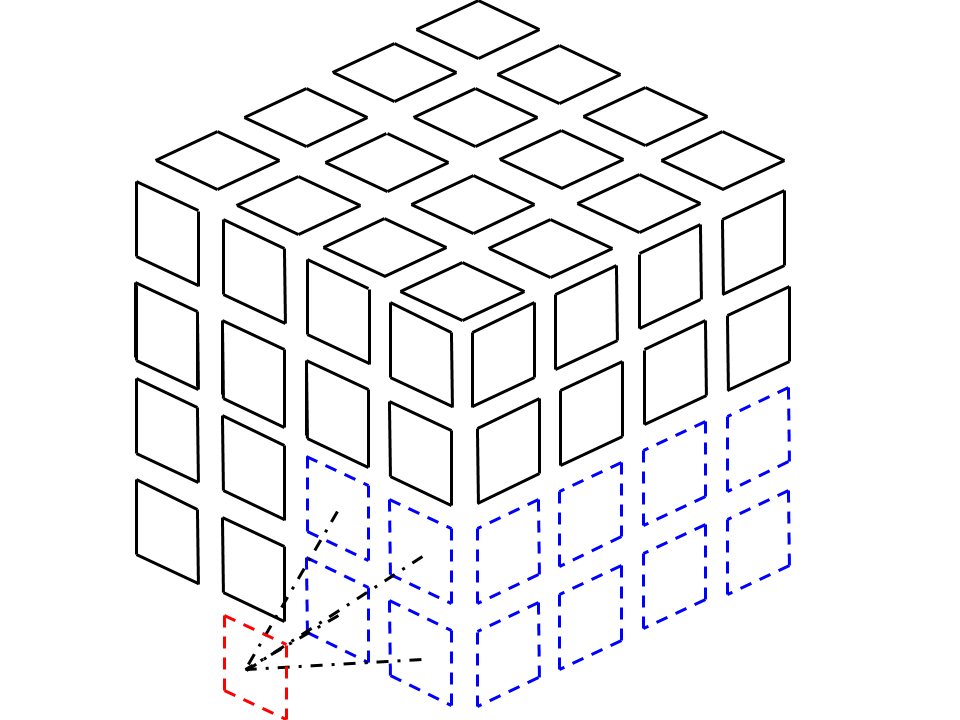
\includegraphics[width=0.333 \textwidth]{images/probabilities}
		\caption{The schematic convergence of predictions from a data cube, where 4 spectras (blue pixels in frequency deep) are analyzed independently, and their results merged into one (red).}
		\label{fig:probabilities}
	\end{center}
\end{figure}

% Pseudo-Code
The algorithm pseudo-code summary can be seen at \ref{alg:algorithm}.

\begin{algorithm}[H]
    \KwData{$data\_cube$, $isotopes\_set$}
        \KwResult{$probability\_predictions$}
            get parameters from $data\_cube$\;
            get input spectra from pixel of $data\_cube$\;
            compute $threshold$ from noise\;
            get $Dictionary$ from $isotopes\_set$\;
            initialize $candidate\_set$ as $[(\;)]$\;
            detect $max\_set$ from spectra\;
            $max_{freq} = max(max\_set)$\;
            \While{$(max_{freq} > threshold)$}{
                ($candidate\_set$).append($max_{freq}$)\;
                subtract Gaussian function at $max_{freq}$\;
	            detect $max\_set$ from residual spectra\;
	            $max_{freq} = max(max\_set)$\;
            }
            recalibrate $Dictionary$ from $candidate\_set$\;
            get $alphas$ from solving sparse coding\;
            compute $probability\_predictions$ from $alphas$\;
            return $probability\_predictions$\;
    \caption{Proposed algorithm}
   	\label{alg:algorithm}
\end{algorithm}


% Specifications of Data Cubes
\subsection{Training/Test set}
For testing purposes, each lines present in the simulated spectras are stored as data cube meta-data, allowing us to evaluate the predictive model and determine metrics to validate predictions.

% How we separated the data
For this, and given the ASYDO simulator capabilities, data cube specifications are separated in two main parameters:
i) signal to noise ratio, using different ALMA bands
ii) fixed/variable width of lines, 
% Different Bands and Variable/Fixed Widths
% Different Band (Noise)
For i), the differences lie in both signal to noise ratio and spectral line density.
ALMA bands 7 and 9 are selected for experiments, and the test consists in 50 cubes, in which half of them are run for different subsets of isotopes present at both ranges 602 - 606 $GHz$ (ALMA band 9) and 275 - 277 $GHz$ (ALMA band 7).
For ii), 50 test run on the same bands, but using variable line width.
Each line width is assigned independently in a range of variation of $(-2, +2) MHz$ from original width.




\section{Experimental results} \label{sec:results}

% Past Tense

\begin{comment}
  - Introduction: What is expected
  - Global Numbers
  - Different Band (Noise)
  - Precision/Recall Graphs
  - Histograms Recall, Precision and F-Score
  
  - Noticeable changes in results
  - Different Width (variable fwmh)
  - Marginal changes in results
  - Border cases not resolved
\end{comment}

%  Introduction: What is expected
In this section, we present and analyze the experimental results.
The idea behind these tests is to simulate data cubes using a known isotope list and then to retrieve of as much elements of the known list as possible.
For each band, the list of all theoretical isotopes in that range are searched in Splatalogue, and a subset of them is selected randomly to simulate data cubes.

\subsection{Measure of accuracy}
To evaluate identification performance, a measure of test accuracy must be design such that we can evaluate percentage of matches between selected words and present lines in simulations.
% Histograms Recall, Precision and F-Score
We use as measures precision, recall and f-score in view of its intuitive ability to explain performance differentiating accuracy from true/false positives/negatives \citep{precision_recall}.
F-score values in table \ref{tab:results} show an overview of obtained results.

Moreover, confusion matrices in figure \ref{fig:confusion_matrix} allow to visually analyze the classifier performance.
The matrices, that corresponds to first 20 experiments at ALMA band 9, show that predictions become less certain at darker zones.
Confusion matrices tends to be higher than wider because of the greater number of false positive predictions over actual isotope lines.
Indicators of performance precision, recall and f-score are calculated from their respective confusion matrices.
The precision/recall curves are shown at figures \ref{fig:results1} and \ref{fig:results2} for ALMA bands 9 and 7 respectively.

\subsection{Prediction results}
Overall results give a f-score above 90\% when the results are filtered for cases in which the lines present in the simulation are higher than 1 MHz.
One might expect higher results in such that cases, but the fact that present lines are not closer does not necessarily simplifies the task.
Theoretical lines keep being very close for some cases and an error margin is expected.

When all results are included, an overall f-score of 82\% is reached, showing that the idea behind this approach is suitable to solve the problem.
In next sections, we will address differences between each group of results.

% Table with Results
\begin{center}
	\begin{table}
		\begin{tabular}{ | l | l | l | }
			\hline
			{\bf ALMA Band/Width } & {\bf Fixed } & {\bf Variable} \\ \hline
			Band 7 & 85.80 \% & 84.79 \% \\ \hline
			Band 9 & 82.05 \% & 78.17 \% \\ 
			\hline
		\end{tabular}
		\caption{ The f-score for different noise level (bands) and width of the lines.}
		\label{tab:results}
	\end{table}
\end{center}

% Noticeable changes in results
\subsection{Signal to noise effect in predictions}
There exists noticeable differences between results for different noise levels.
For band 9, an overall of 80\% shows that both the higher noise and density affect prediction accurately.
On the other hand, band 7 reaches an overall of 85\%, although there are not appreciable differences between the measures distribution as can be seen in both figures \ref{fig:hist1} and \ref{fig:hist2}.

Figures \ref{fig:results1} and \ref{fig:results2} show an intuition of exchange ratio between true positive and false negatives.
Precision/recall curve at band 7 has a better trade-off as its slope is smaller,  and this is reflected in better prediction of true positives without increasing false positives.

\subsection{Variable width effect in predictions}
% Different Width (variable fwmh)
To test more realistic cases, where line width variates randomly, there is a small difference of almost 1\% for band 7.
Not so at band 9, where a difference of 4\% shows that higher density of lines is affected by the randomness of lines's width.
Also, figures \ref{fig:hist1} and \ref{fig:hist2} shows the differences between accuracy measures for both cases, being the fixed width focused in a smaller range than variable width results.

% Example of Modified Confusion Matrix
\begin{figure}
	\begin{center}
		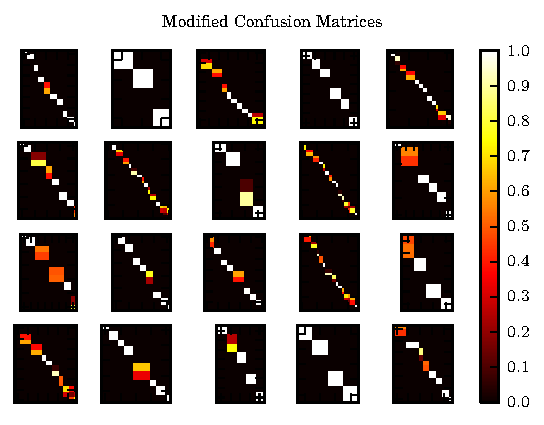
\includegraphics[width=0.45 \textwidth]{images/confusion_matrix}
		\caption{ Modified confusion matrices for 20 experiments for data cubes with fixed line width at band 9. Predictions tend to be on the diagonal because of the algorithm preference for closer theoretical line's frequencies.}
		\label{fig:confusion_matrix}
	\end{center}
\end{figure}

% Precision/Recall Curve
\begin{figure}[H]
	\begin{center}
		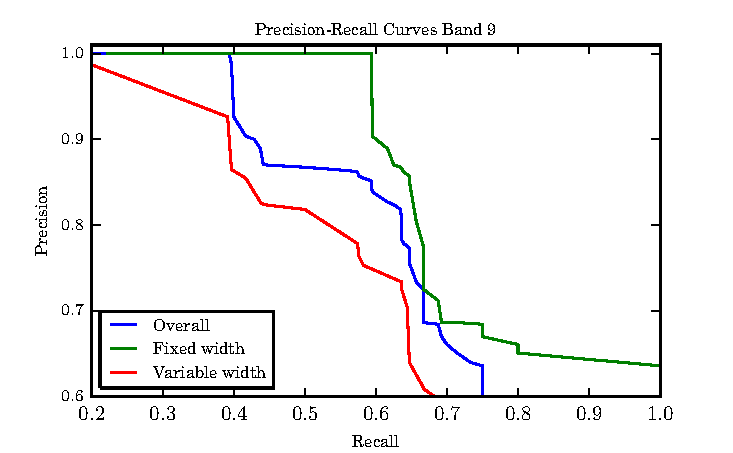
\includegraphics[width=0.45\textwidth]{images/results1}
		\caption{ The measures of accuracy, precision and recall obtained for fixed line width cubes, variable line width and overall results for ALMA band 9.}
		\label{fig:results1}
	\end{center}
\end{figure}

\begin{figure}[H]
	\begin{center}
		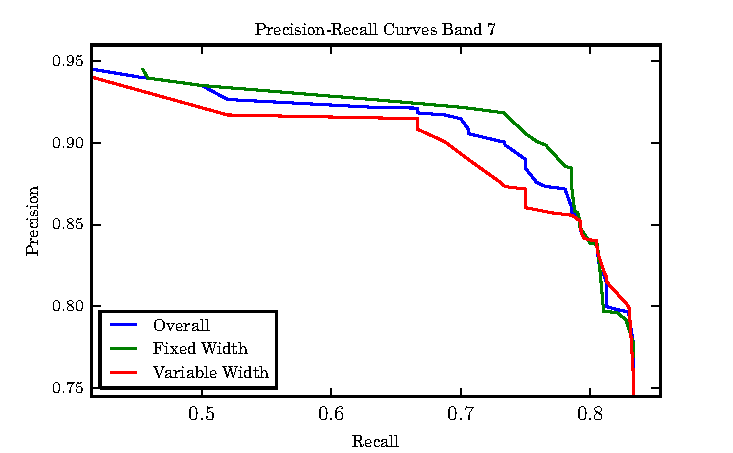
\includegraphics[width=0.45\textwidth]{images/results2}
		\caption{ The measures of accuracy, precision and recall obtained for fixed line width cubes, variable line width and overall results for ALMA band 7. }
		\label{fig:results2}
	\end{center}
\end{figure}

% Histograms of results Fixed Width
\begin{figure}[H]
	\begin{center}
		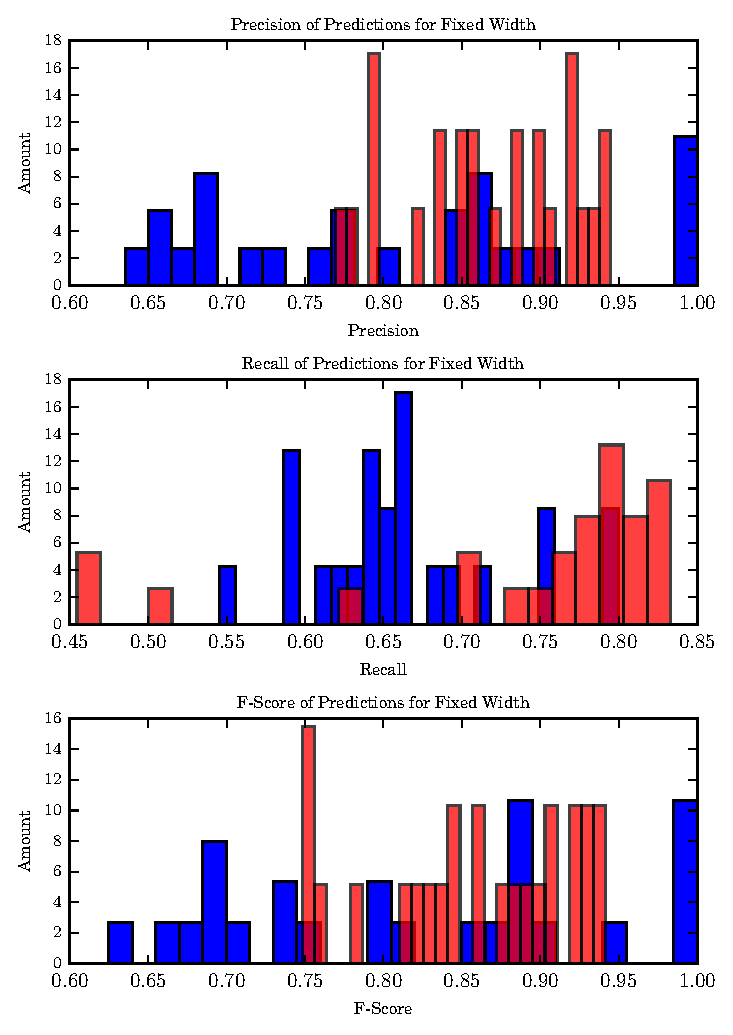
\includegraphics[width=0.45\textwidth]{images/hist1}
		\caption{ Histograms of results obtained for the test performed for precision, recall and f-score for fixed line width (red) vs variable line width (blue) in Band 9.}
		\label{fig:hist1}
	\end{center}
\end{figure}

\subsection{Complex cases}
%  %  Blending case
We focus our analysis on complex cases and show examples of how the algorithm handle them.

For blending cases, the algorithm gives a probability distribution of potential overlapped lines. In general, when blending exists, one of the predicted lines losses certainty, as showed in figure \ref{fig:blending}.

\begin{figure}[H]
	\begin{center}
		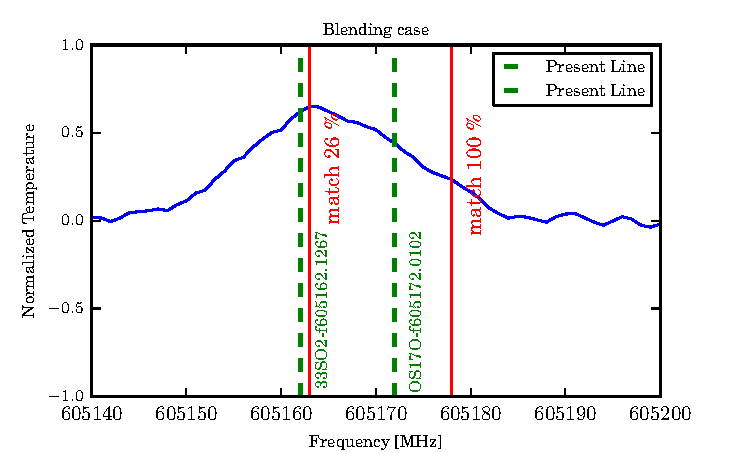
\includegraphics[width=0.45\textwidth]{images/blending}
		\caption{ Blending case }
		\label{fig:blending}
	\end{center}
\end{figure}

% Histograms of results Variable Width
\begin{figure}[H]
	\begin{center}
		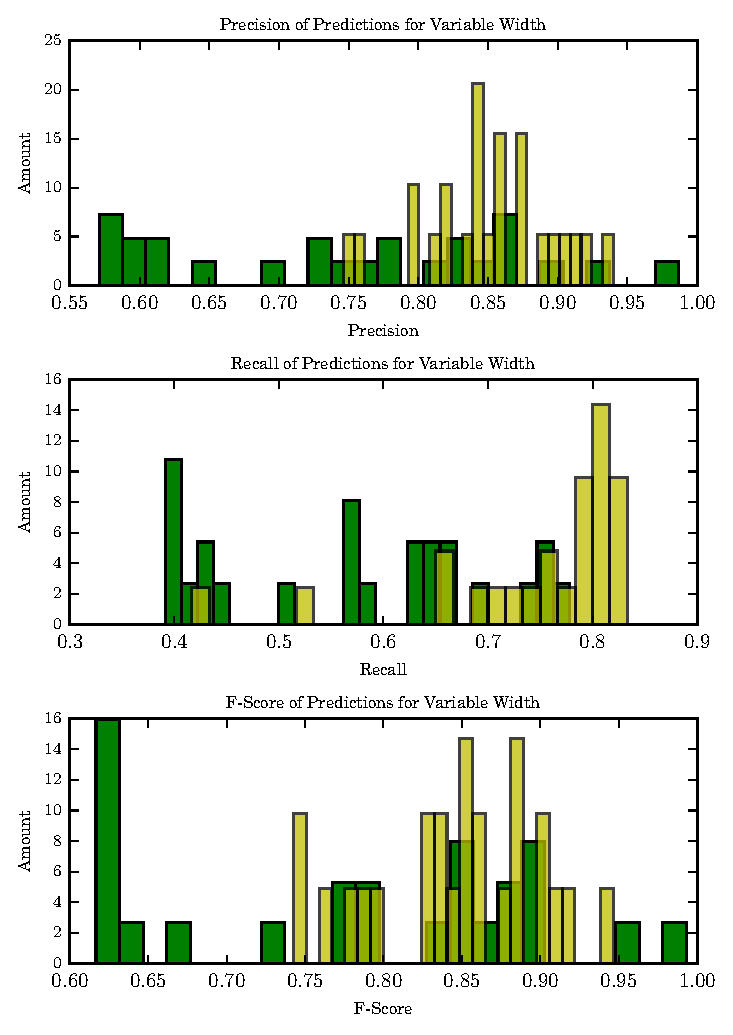
\includegraphics[width=0.45\textwidth]{images/hist2}
		\caption{ Histograms of results obtained for the test performed for precision, recall and f-score for fixed line width (yellow) vs variable line width (green) in Band 7.}
		\label{fig:hist2}
	\end{center}
\end{figure}


% Double peaks for single Line
False double peaks product of artifacts are handled by the algorithm and it determines the correct lines among false peaks, as showed in figure \ref{fig:doublepeak}.

\begin{figure}[H]
	\begin{center}
		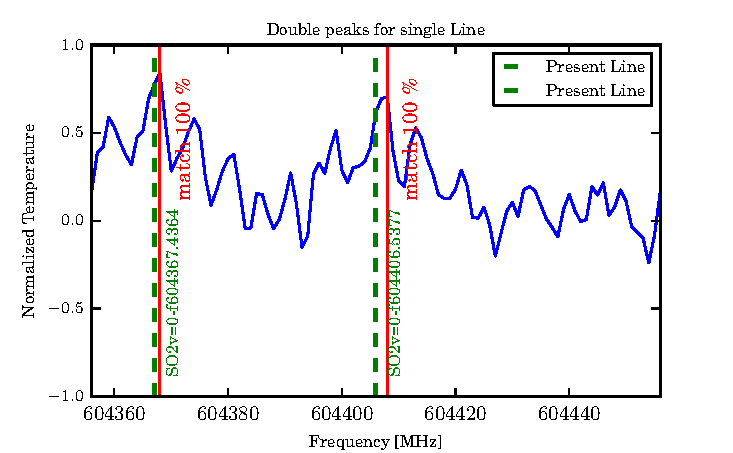
\includegraphics[width=0.45\textwidth]{images/doublepeak}
		\caption{ Double peaks for single Line }
		\label{fig:doublepeak}
	\end{center}
\end{figure}

\subsection{Real Data}

Additionally to synthetic results, real data from ALMA is used to test the algorithm's behavior.
The experiments consists in the analysis over product cubes to predict isotopes associated to molecules observed for each cube.
The used cubes are product of a deconvolution using CASA task CLEAN as explained at \cite{higuchi_iras_2015}.

\begin{figure}[H]
	\begin{center}
		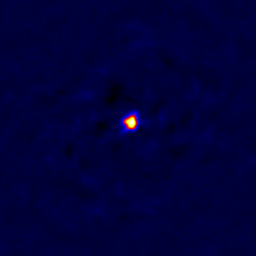
\includegraphics[width=0.225\textwidth]{images/ds9}
		\caption{ Example of used data cubes, slice of $IRAS16547-4247\_Jet\_CH3OH7-6.clean$ from project ALMA project \#2011.0.00419.S.  }
		\label{fig:ds9}
	\end{center}
\end{figure}

In this case, the high density of theoretical frequencies plays a major role in the difficulty of the prediction.
With synthetically data, a subset of isotopes were selected, but with real data, all the Splatalogue lines were include to test the process in a real world scenario.

The algorithm is able to predict lines for $CH_3OH_7 (7-6)$, but the algorithm is not able to predict other isotopes of interest.
The algorithm gives a list and a probability of presence in each cube. In table \ref{tab:real-results} we present only predicted frequencies associated to the isotopes of interest.

The process of the predicted isotope can be seen in figure \ref{fig:experiment}.
The amount of theoretical frequencies that must be filtered in order to make a prediction can be seen explicitly in the visual representation of the process.

% Real Data
\begin{center}
	\begin{table}
		\begin{tabular}{ | l | l | l | }
			\hline
			{\bf File } & {\bf Predicted frequencies }  \\ \hline
			$13CH3CN19-18$ 				& - \\ \hline
			$CH3OH7-6$ 					& 338486.337 and 338486.337, \\
					 					& 338583.195, 338639.939 \\ \hline
			$CS_v1\_7-6$ 				& - \\ \hline
			$SO2$ 		 				& -  \\ \hline
			$SO2-28\_2\_26-28\_1\_27$ 	& -   \\ \hline
			\hline
		\end{tabular}
		\caption{ Predicted frequencies associated to the molecules of interest for each clean cube for ALMA project \#2011.0.00419.S.}
		\label{tab:real-results}
	\end{table}
\end{center}

\begin{figure}
	\begin{center}
		% 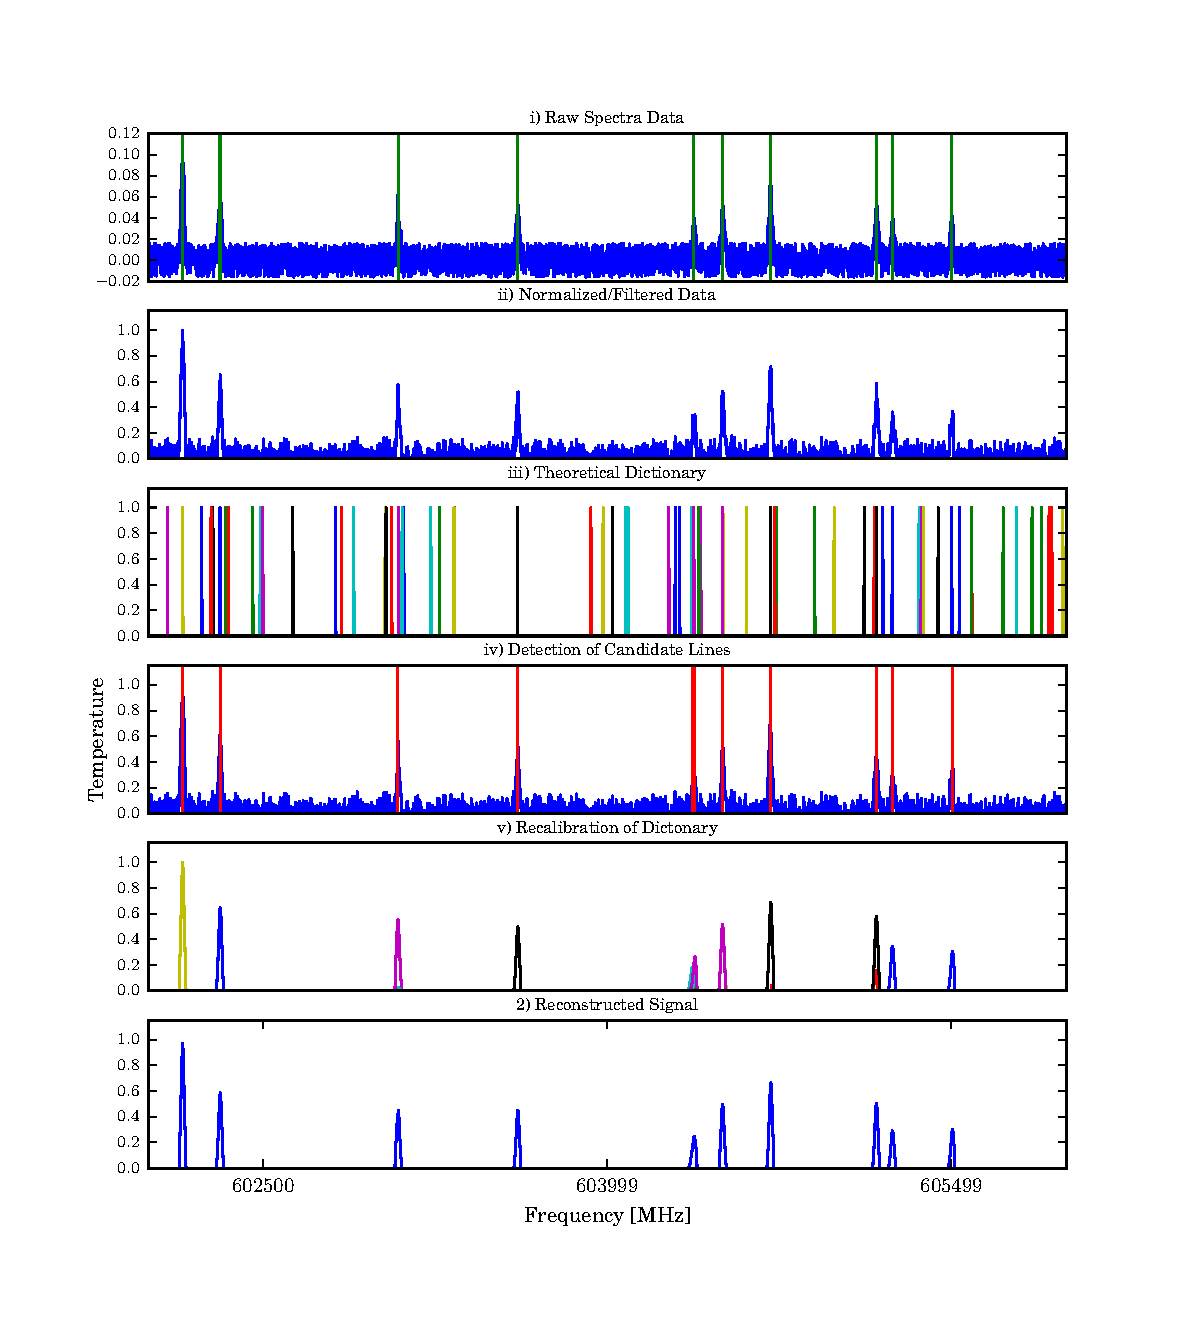
\includegraphics[width=\textwidth]{images/process}
		\label{fig:experiment}	
				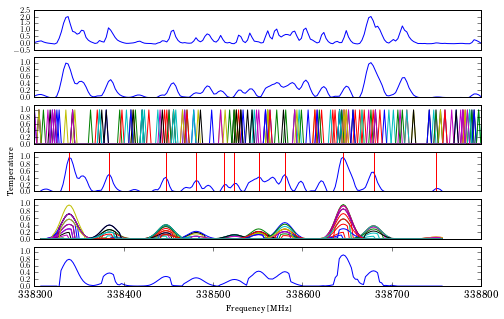
\includegraphics[width=0.5\textwidth]{images/experiment}%
		\caption{Data cube example following the steps previously explained.}
	\end{center}
\end{figure}








\section{Conclusion} \label{sec:conclusions}

% Present Tense %
\begin{comment}
  - Remember hypothesis
  - Results support hypothesis
  - Reached objective proposed in the focus of the problem
  - With some exceptions, results archived
  - Extensibility
  - Next steps
\end{comment}

% Summary: Summarizing (briefly) from specific to general
Our approach to identify emission lines is the reconstruction of an input signal.
The combination of representative basis vectors allows us to predict the presence of isotopes lines along the wavelength spectra.
The set of coefficients used to reconstruct the signal give us an idea of the presence of each isotope line.

This process can be summarized as two main hypothesis:
i) a set of basis vectors representing theoretical lines allows to reconstruct an input spectra, and
ii) the used combination of basis vectors gives useful information to identify the presence of emission lines along the spectra.

% Confirm the topic in the introduction
Results has shown support for the hypothesis, but leaves room for improvements that increases its possibilities given the near arrival of new real data.
This data will allow to future investigators to train models and capture actively the patterns in data, its correlations and hidden latent variables.

Sparse coding technique allows to identify isotope lines even when blending is present.
This gives a notion of the molecular composition of the astronomical object and allows astronomers to focus on complex cases.

% Extensibility
A major issue in the algorithm elaboration is the lack of information about relative intensities relationships and the co-presence dependence for lines of the same isotope.
That makes the algorithm to try to find each isotope line independently.
Future extensibility from real data can be:
i) the inclusion of relationship between temperatures of lines belonging to the same isotope, and 
ii) to learn the dependence of co-presence of lines, not just for the same isotopes, but for all molecules.
On that line, theoretical lines belonging to unknown molecules are an interesting case to cover.
The possible relationships between unidentified lines and known molecules could be used as a way to assign unknown lines to an isotope. 

% Finally, how the topic relates to its context
% Next steps
The solution proposed resulted in a first approach to solve this problem.
Real data will give to researchers new tools to analyze and develop more complex models to make use of patterns that simulations do not allow us to use.
Certainly, future work can make use of a big amount of data available with the forward of ALMA project to apply more complex word representations and signal reconstruction models.

\section*{Acknowledgments}

This investigation is supported by Vicerrectoría de Investigaci\'on (VRI) from Pontificia Universidad Cat\'olica de Chile.
Institute of Applied Computer Science at Harvard University.

This  work  is  funded  by  project  FONDEF  D11I1060:  Development  of  an  astro-informatics  platform  for management and intelligent analysis of large-scale data, a collaborative project between several Chilean universities in order to create a Chilean virtual observatory, called Observatorio Virtual Chileno (ChiVO)
\footnote{\url{http://www.chivo.cl}}.

This paper makes use of the following ALMA data: ADS/JAO.ALMA\#2011.0.00419.S. ALMA is a partnership of ESO (representing its member states), NSF (USA) and NINS (Japan), together with NRC (Canada), NSC and ASIAA (Taiwan), and KASI (Republic of Korea), in cooperation with the Republic of Chile. The Joint ALMA Observatory is operated by ESO, AUI/NRAO and NAOJ.

\thispagestyle{empty}

\addcontentsline{toc}{section}{References}
\bibliography{paper-meta}
\bibliographystyle{plainnat}

\end{document}